\documentclass{article}
\usepackage{amsmath}
\usepackage{array}
\usepackage{tabularx}
\usepackage{hyperref}
\usepackage{xcolor}
\usepackage[UTF8]{ctex}
\usepackage{fullpage}
\usepackage{float}
\usepackage{graphicx}
\usepackage{subcaption}
\usepackage{lipsum}

\hypersetup{
  colorlinks=true, 
  linkcolor=blue, 
  citecolor=blue, 
  urlcolor=blue,
  pdfborder={0 0 0},
  pdfborderstyle=/S/U/W 0
}

\title{学习回顾}
\author{蔡鞅}
\date{\today} 

\begin{document}
	
	\maketitle 

  \begin{abstract}
    致魏老师:

    在之前CNN的学习过程当中,我发现自己对于神经网络模型内部的结构了解较为匮乏,
    以至于难以继续学习深入的内容。
    5月份到7月份期间,我学习了深度学习当中的基本概念,例如损失函数、激活函数、反向传播、优化器,
    以及模型训练当中的相关技巧,例如Batch Normalization、Weight Sharing、Truncated Loss。
    此外,我还了解了一些经典的卷积神经网络结构,例如AlexNet、VGGNet、GoogleNet,
    以及经典的循环神经网络结构,例如RNN、GRU、LSTM。
    
    最后,我利用PyTorch动手实现了一些结构较为简单的模型,并用CIFAR-10数据集和China Daily上的一些文章作为训练集,
    开展了一些小实验,并用LaTex撰写了这篇实验笔记。
    
    由于训练模型的硬件条件有限(没有AMD或者Nvdia的GPU),数据集较小,循环神经网络的训练效果较为不理想。
    此外,我个人在原始数据的处理以及格式转换上仍然缺乏一定的经验和能力,希望能够通过后续的学习弥补不足。

    祝您工作顺利!
  \end{abstract}

	\newpage
  \section{ResNet}
ResNet的核心就是对每一个残差块,将输入与卷积后的输出相加后再传递激活函数,
而并非只将输出传递给激活函数,从而解决了模型较深时梯度消失的问题。
残差块的典型结构如图\ref{fig:ResNetArchitecture}所示。

\begin{figure}[H]
    \begin{subfigure}[c]{0.45\textwidth}
        \centering
        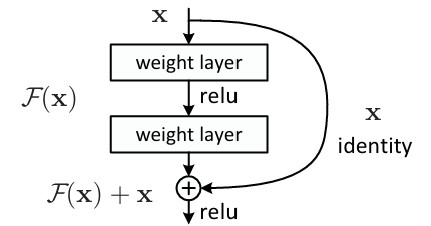
\includegraphics[width=0.8\textwidth]{./figures/ResNetArchitecture.jpg}
        \caption{ResNet残差块结构}
        \label{fig:ResNetArchitecture}
    \end{subfigure}
    \hfill
    \begin{subfigure}[c]{0.45\textwidth}
        \centering
        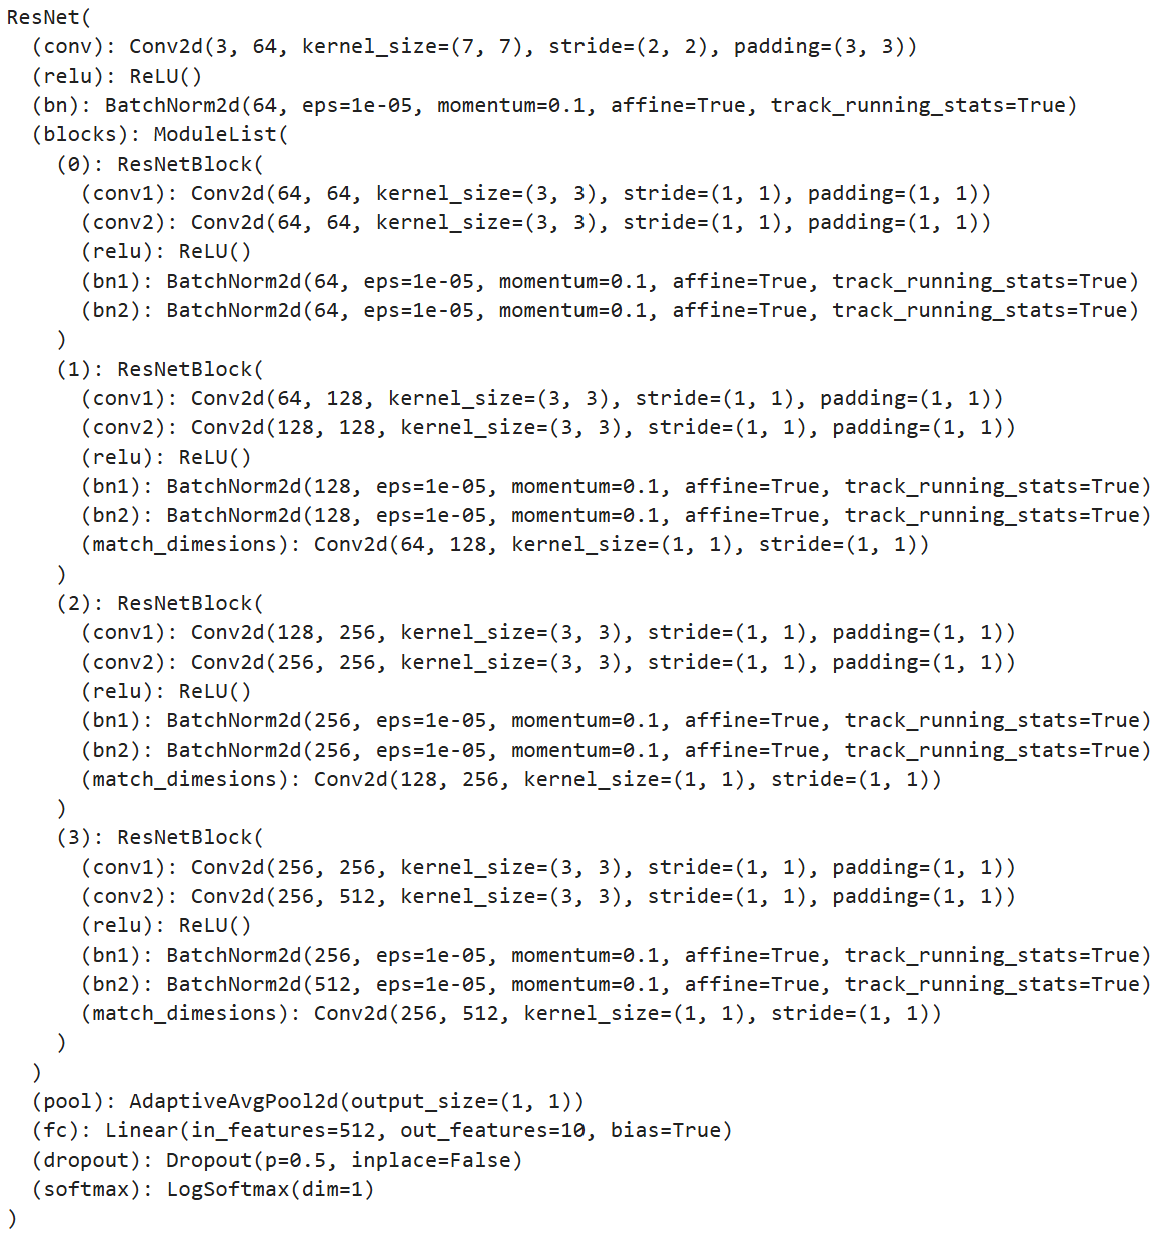
\includegraphics[width=0.8\textwidth]{./figures/MyResNet.png}
        \caption{实验采用的ResNet结构}
        \label{fig:MyResNet}
    \end{subfigure}
    \caption{模型结构}
    \label{fig:Architectures}
\end{figure}

本次实验的ResNet结构如图\ref{fig:MyResNet}所示。
每一个残差块当中都会根据输入和输出的尺寸进行判断。
如果输入和输出的尺寸不同,残差块当中会添加一个额外的卷积层,其卷积核大小为1。
输入通过该卷积层后与输出尺寸相同,从而能够完成相加操作。

实验利用CIFAR-10数据集来训练模型,损失曲线如图\ref{fig:resnetlosshistory}所示,
训练过程当中,模型在训练集上和测试集上的准确率曲线如图\ref{fig:resnetmetrics}所示。

\begin{figure}[H]
    \begin{subfigure}[c]{0.45\textwidth}
        \centering
        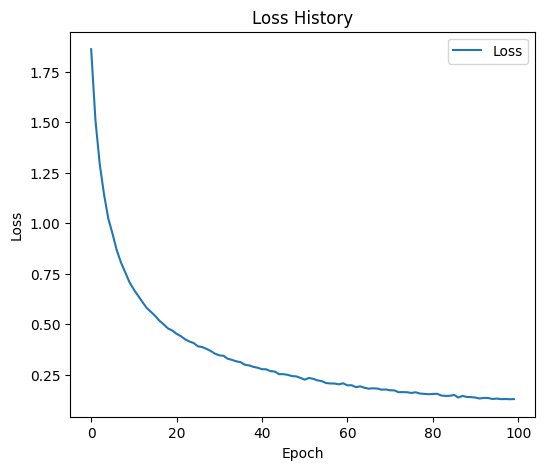
\includegraphics[width=\textwidth]{../output/resnet/loss_history.png}
        \caption{损失曲线}
        \label{fig:resnetlosshistory}
    \end{subfigure}
    \hfill
    \begin{subfigure}[c]{0.45\textwidth}
        \centering
        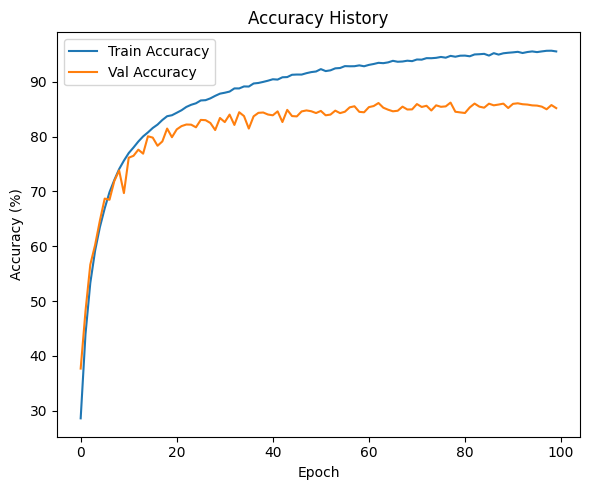
\includegraphics[width=\textwidth]{../output/resnet/metrics.png}
        \caption{准确率曲线}
        \label{fig:resnetmetrics}
    \end{subfigure}
\end{figure}

最后将模型第一个卷积层可视化。

\begin{figure}[H]
    \centering
    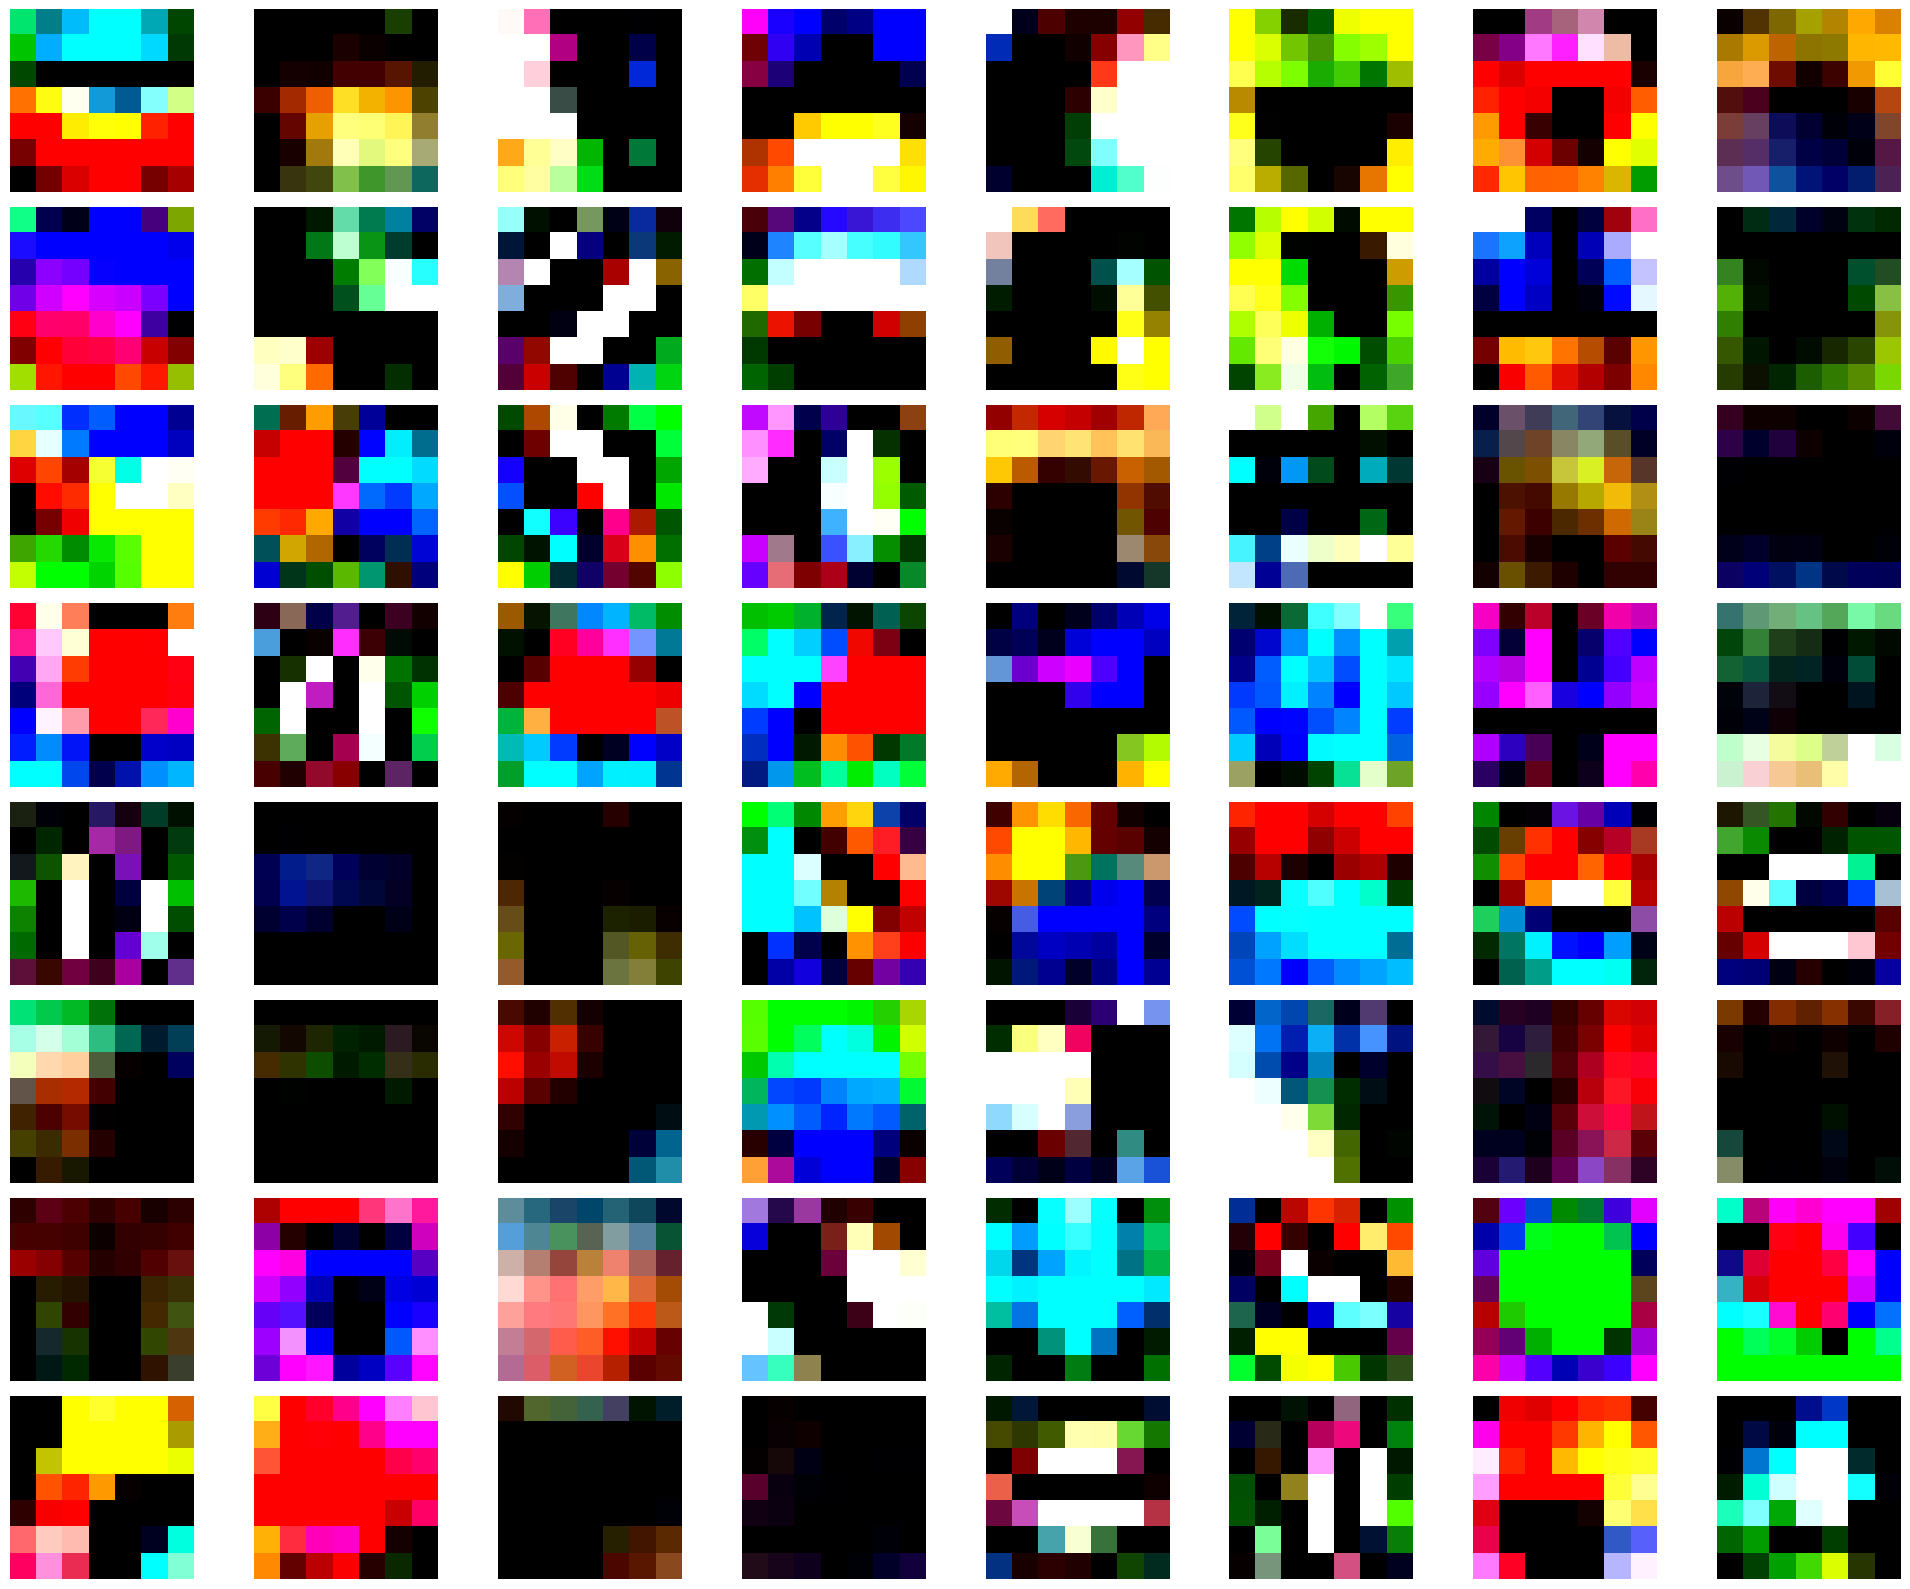
\includegraphics[width=0.5\textwidth]{../output/resnet/conv1.png}
    \caption{模型第一个卷积层}
\end{figure}
  \section{RNN}
    RNN的总体结构如图\ref{fig:rnnarchitecture}所示。

    \begin{figure}[H]
        \centering
        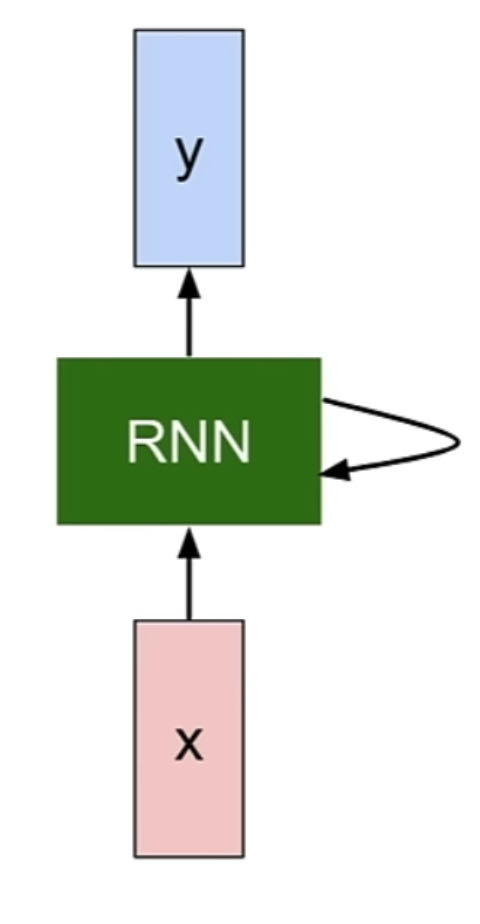
\includegraphics[width=0.07\textheight]{./figures/rnnarchitecture.jpg}
        \caption{RNN结构}
        \label{fig:rnnarchitecture}
    \end{figure}

    在$t$时刻,通常用$h_t$代表隐藏层的状态,$x_t$代表输入,$y_t$代表输出。
    于是隐藏层的状态更新可以用

    \begin{equation}
        h_t = f_W (h_{t-1}, x_t)
    \end{equation}
    来表达。一个比较简单的例子为双曲正切函数,即$h_t = \tanh (W_{hh} h_{t-1} + W_{xh} x_t)$。

    对于不同的场景,RNN的计算图有不同的形式。
    例如,生成图像标题的RNN计算图为单一输入到多输出,
    机器翻译的RNN计算图为多输入到多输出。
    本次实验采用的RNN结构为单一输入到单一输出,
    利用每一个时间步的输入来预测下一个时间步的输出。
    原始输入节选自China Daily在2024年7月25日发布的
    World hails success of historic Palestinian unity declaration
    和
    Expert: Pursuit of new tech should be sensible,
    利用One-Hot编码处理后训练RNN模型,得到的损失曲线如图\ref{fig:RNNlosshistory}所示,
    权重矩阵热力图如图\ref{fig:rnnweightmatrix}所示。

    \begin{figure}[H]
        \centering
        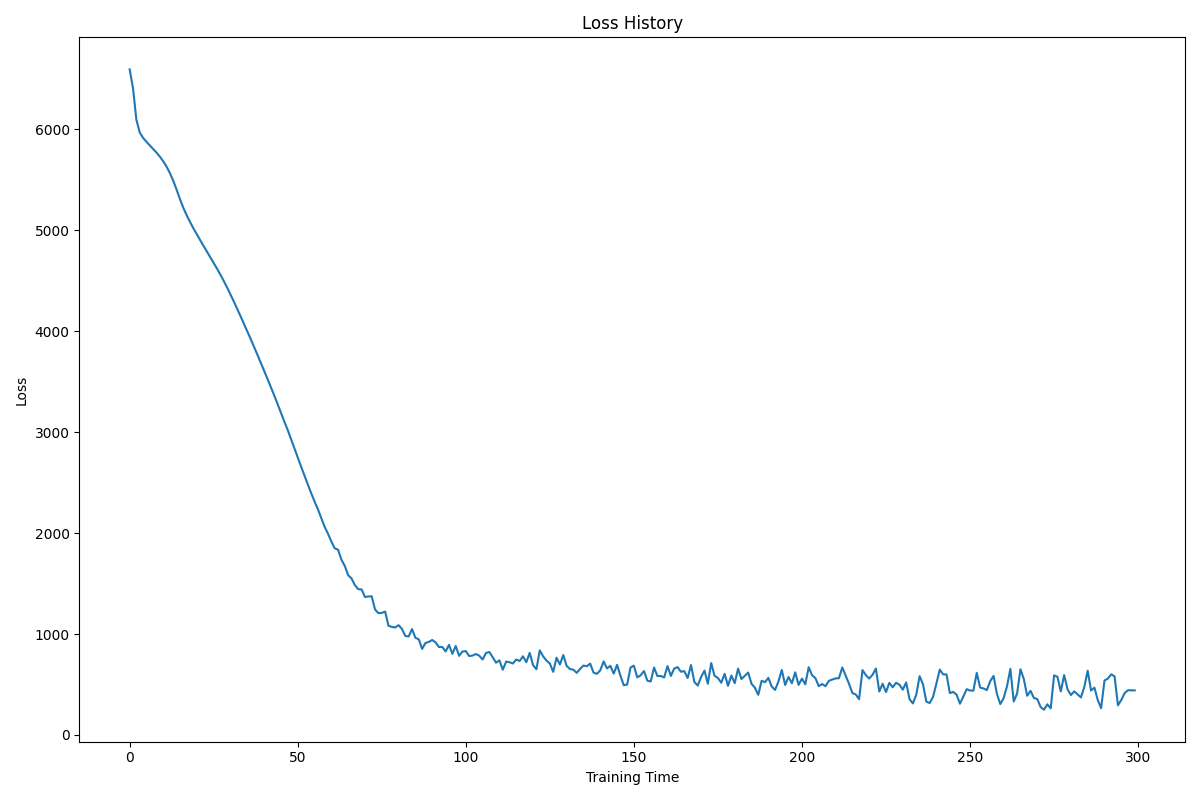
\includegraphics[width=0.7\linewidth]{../output/rnn/no scheduler/rnnloss.png}
        \caption{RNN损失曲线}
        \label{fig:RNNlosshistory}
    \end{figure}

    \begin{figure}[H]
        \centering
        \begin{subfigure}{0.3\textwidth}
            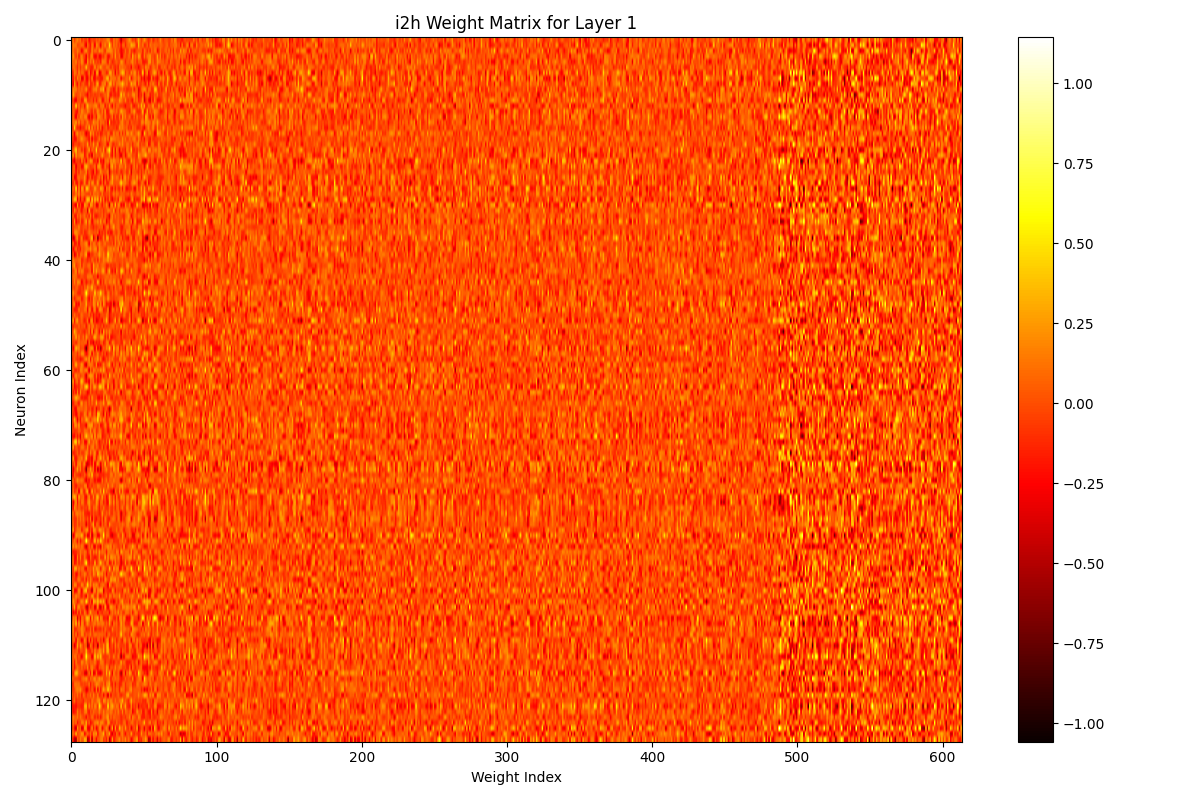
\includegraphics[width=\linewidth]{../output/rnn/no scheduler/Weight Matrix for Layer 1.png}
            \caption{第1层}
            \label{fig:rnnweightmatrixforlayer1}
        \end{subfigure}
        \hfill
        \begin{subfigure}{0.3\textwidth}
            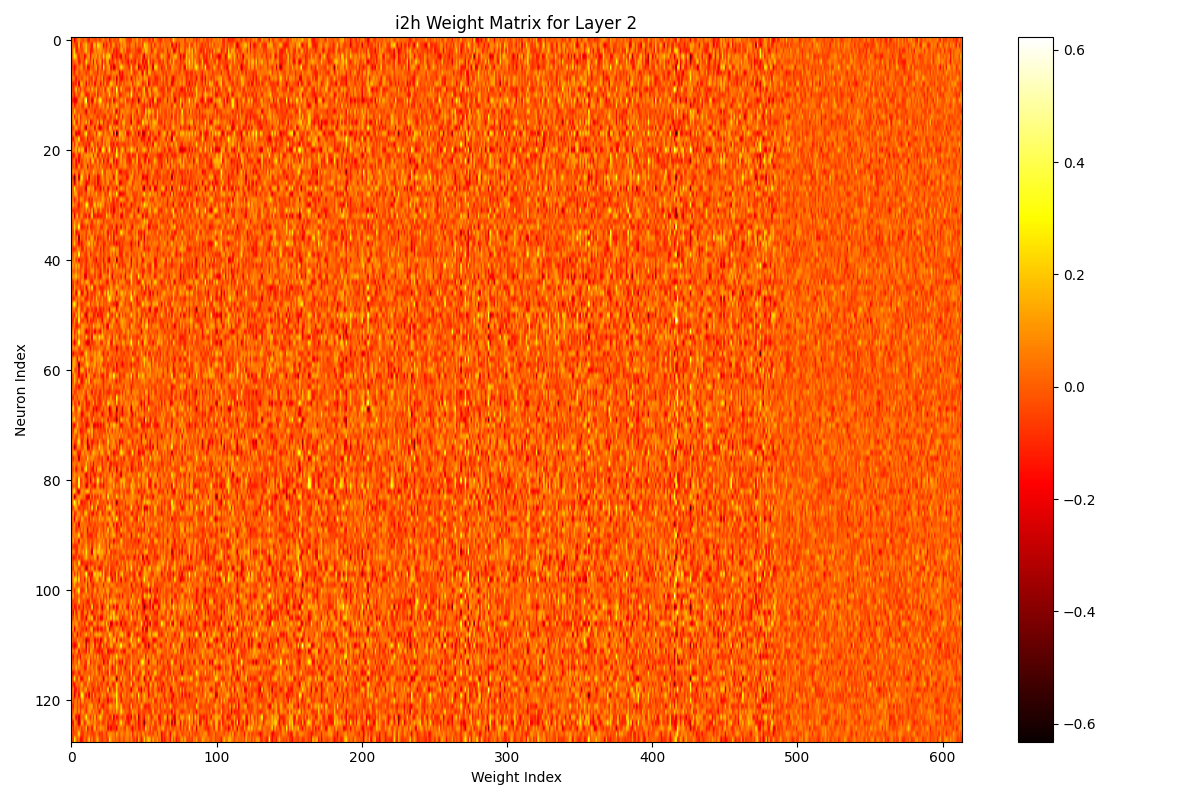
\includegraphics[width=\linewidth]{../output/rnn/no scheduler/Weight Matrix for Layer 2.png}
            \caption{第2层}
            \label{fig:rnnweightmatrixforlayer2}
        \end{subfigure}
        \hfill
        \begin{subfigure}{0.3\textwidth}
            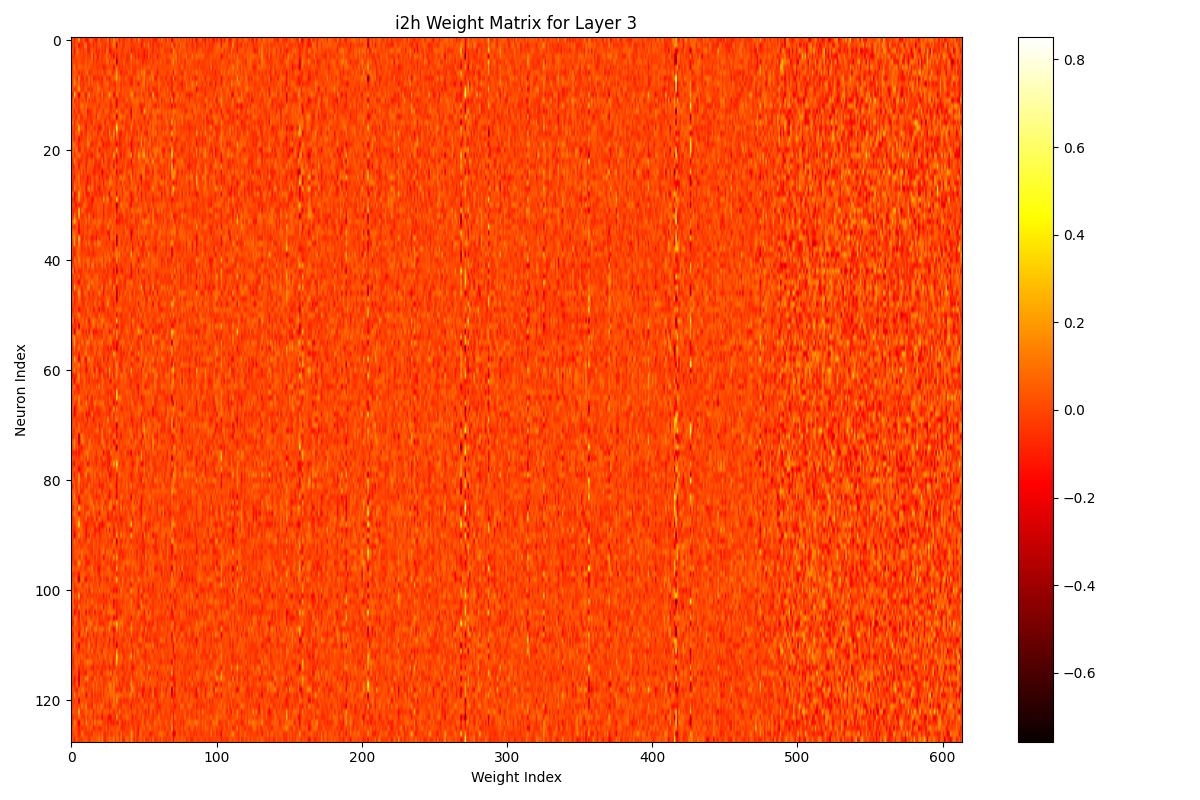
\includegraphics[width=\linewidth]{../output/rnn/no scheduler/Weight Matrix for Layer 3.png}
            \caption{第3层}
            \label{fig:rnnweightmatrixforlayer3}
        \end{subfigure}
        \caption{RNN隐藏层权重矩阵}
        \label{fig:rnnweightmatrix}
    \end{figure}

    注意到损失值在经历多轮训练之后并未完全收敛,损失曲线存在较多的毛刺,模型出现了局部退化的现象。
    此处可以采用学习率调度机制来改善训练过程,
    在模型的训练过程中添加ReduceLROnPlateau调度器,
    factor设置为0.1,mode设置为min,patience设置为5,
    处理后得到的损失曲线如图\ref{fig:RNNlosshistorywithscheduler}所示,
    权重矩阵热力图如图\ref{fig:rnnweightmatrixwithscheduler}所示。

    \begin{figure}[H]
        \centering
        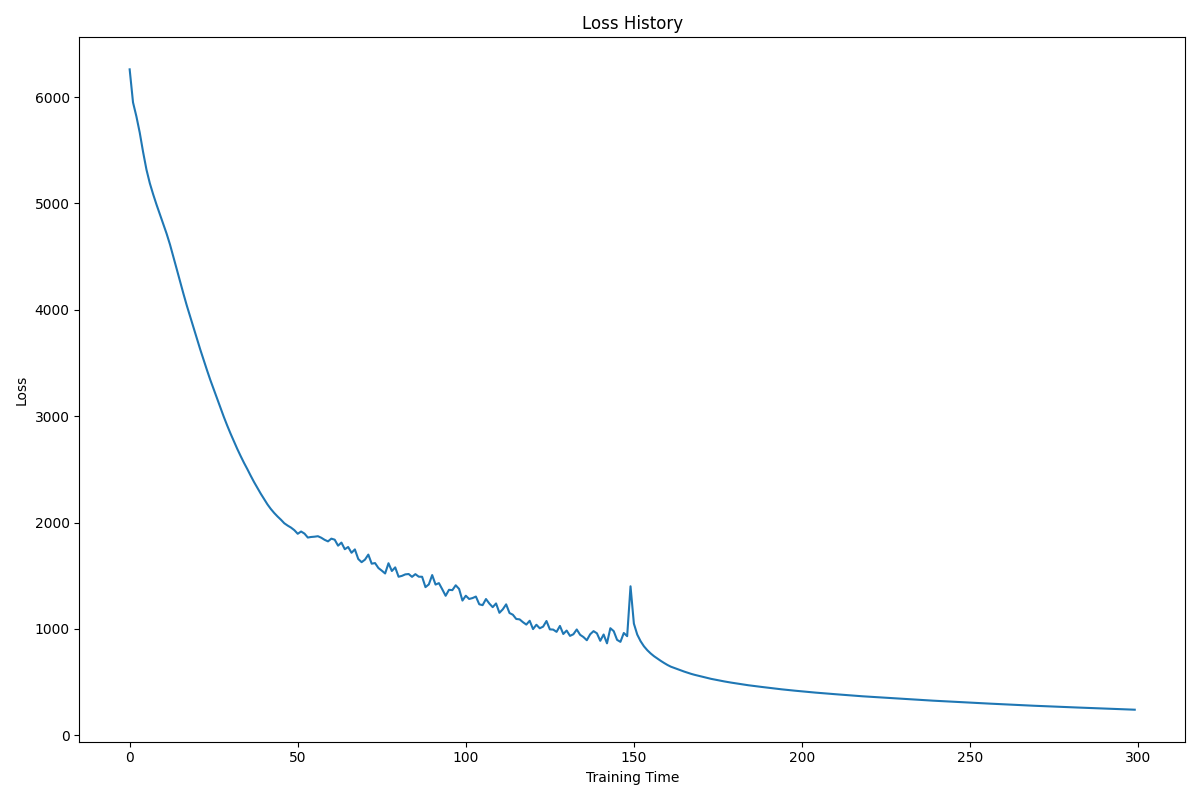
\includegraphics[width=\linewidth]{../output/rnn/with scheduler/rnnloss.png}
        \caption{RNN损失曲线}
        \label{fig:RNNlosshistorywithscheduler}
    \end{figure}

    \begin{figure}[H]
        \centering
        \begin{subfigure}{0.3\textwidth}
            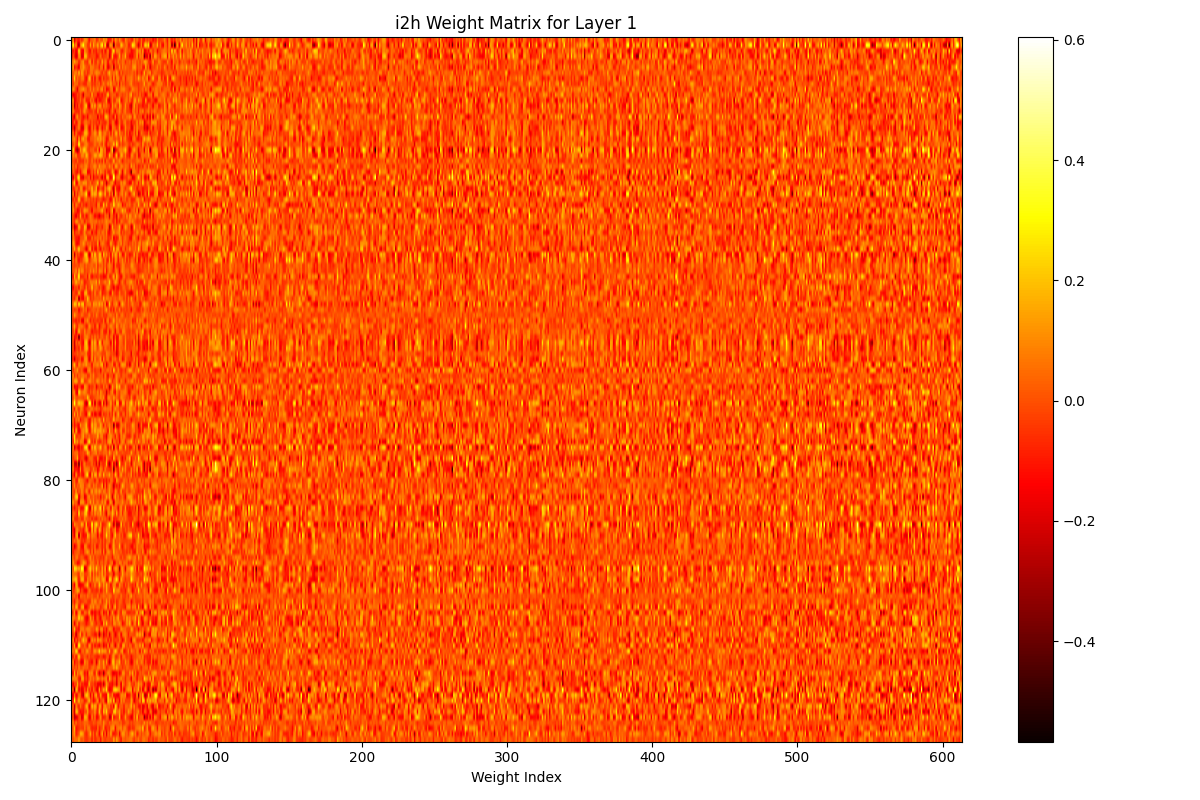
\includegraphics[width=\linewidth]{../output/rnn/with scheduler/Weight Matrix for Layer 1.png}
            \caption{第1层}
            \label{fig:rnnweightmatrixforlayer1withscheduler}
        \end{subfigure}
        \hfill
        \begin{subfigure}{0.3\textwidth}
            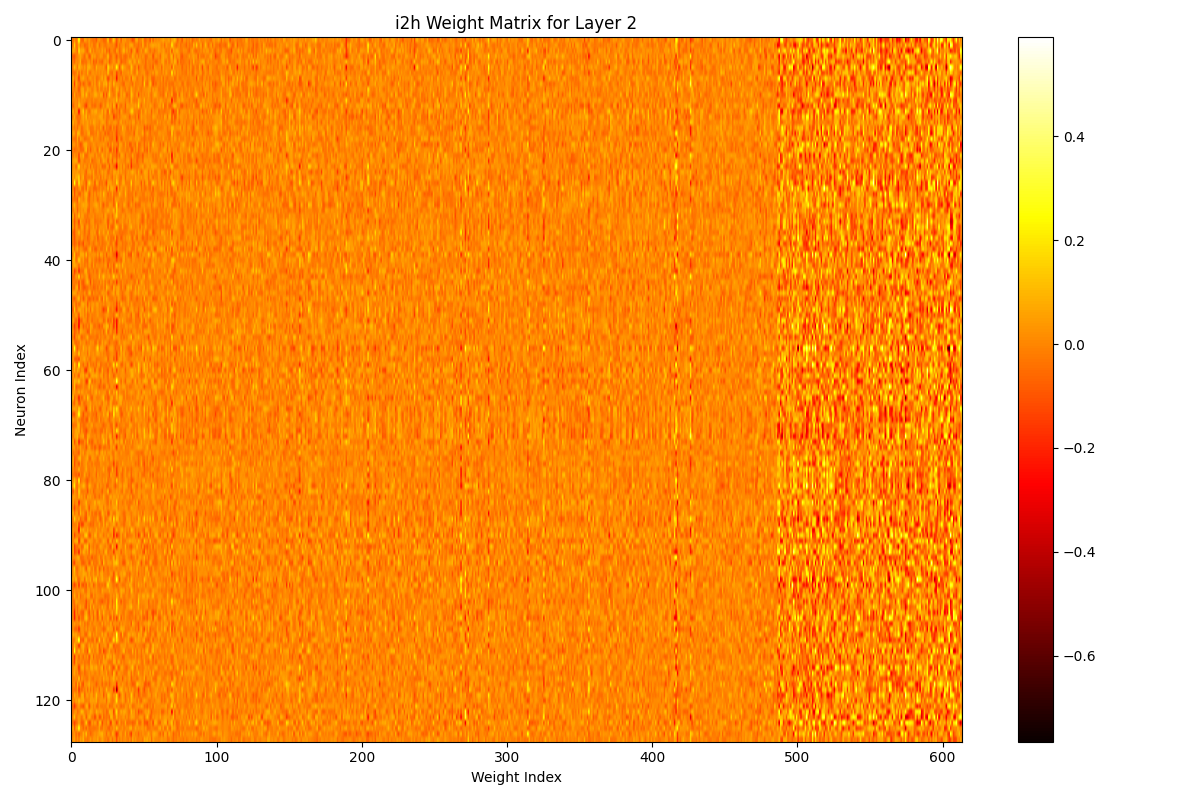
\includegraphics[width=\linewidth]{../output/rnn/with scheduler/Weight Matrix for Layer 2.png}
            \caption{第2层}
            \label{fig:rnnweightmatrixforlayer2withscheduler}
        \end{subfigure}
        \hfill
        \begin{subfigure}{0.3\textwidth}
            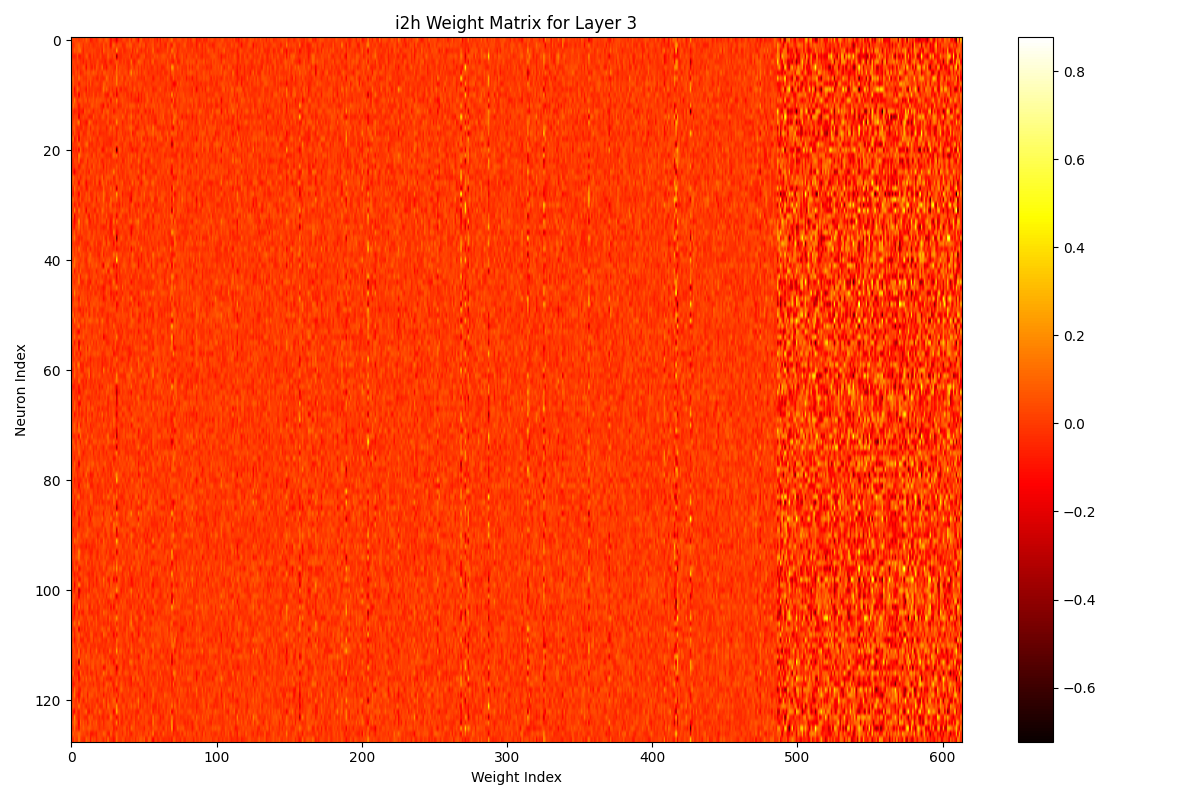
\includegraphics[width=\linewidth]{../output/rnn/with scheduler/Weight Matrix for Layer 3.png}
            \caption{第3层}
            \label{fig:rnnweightmatrixforlayer3withscheduler}
        \end{subfigure}
        \caption{RNN隐藏层权重矩阵}
        \label{fig:rnnweightmatrixwithscheduler}
    \end{figure}

    分别调用两次训练后的RNN模型,输入提示词china后,设置生成文本长度为100,得到的结果如图\ref{fig:rnntext-comparison}所示。

    \begin{figure}[H]
        \centering
        \begin{subfigure}[b]{0.45\textwidth}
            \textit{"china for facilitating talks among hamas fatah and 12 other palestinian factions anwar said that have different competitive advantages to play to china's people to leverage the formation of new production factor lin further said china needs to reform its financial system to better mobilize financial resources for supporting innovations while implementing fiscal reforms to better balance spending responsibilities between local and central governments encouraging the development of venture capital and patient capital will be important improvements he said li dongsheng founder and chairman of chinese consumer electronics maker tcl technology group corp said china's new growth drivers come from industrial"}
            \caption{不使用调度器}
            \label{fig:rnntextnoscheduler}
        \end{subfigure}
        \hfill
        \begin{subfigure}[b]{0.45\textwidth}
            \textit{"china must stand in solidarity with the palestinian people and urge israel to end its brazen violence which has destroyed gaza and killed around 40000 innocent palestinians in the past 10 months sharif said pakistan reaffirms its unwavering support for the palestinian cause and reiterates its call for a two-state solution that creates an independent state of palestine with pre-1967 borders he added the foreign ministry of turkiye welcomed in a statement the gathering of palestinian factions has been broadly hailed as an exceptional success in china's diplomatic efforts to create conditions for lasting peace in gaza and urged nations that"}
            \caption{使用调度器}
            \label{fig:rnntextwithscheduler}
        \end{subfigure}
        \caption{RNN生成文本比较}
        \label{fig:rnntext-comparison}
    \end{figure}
	\section{LSTM}
    RNN模型存在的主要问题是,当输入序列过长时,反向传播的计算量过大,实际应用当中大多使用Truncated Backpropagation来处理此问题。
    当然,更好的方法是使用LSTM模型。

    LSTM在RNN的基础上多添加了一个隐藏层cell state,通常用$c_t$来表示,
    此外LSTM还有对应的门控机制来更新模型当中的两个隐藏层,如公式\ref{eq:lstm}所示。
    \begin{equation}
        \begin{aligned}
            \begin{pmatrix}
                i \\ 
                f \\ 
                o \\ 
                g
            \end{pmatrix}
            &=
            \begin{pmatrix}
                \sigma \\ 
                \sigma \\ 
                \sigma \\ 
                \tanh
            \end{pmatrix}
            W
            \begin{pmatrix}
                h_{t-1} \\
                x_t
            \end{pmatrix} \\
            c_t &= f \odot c_{t-1} + i \odot g \\
            h_t &= o \odot \tanh(c_t)
        \end{aligned}
        \label{eq:lstm}
    \end{equation}
    对应的传播模型如图\ref{fig:lstmarchitecture}所示。
    可见,LSTM在反向传播的过程中只需对$c_t$的相关参数进行计算,大幅减少了反向传播的计算量。

    \begin{figure}[H]
        \centering
        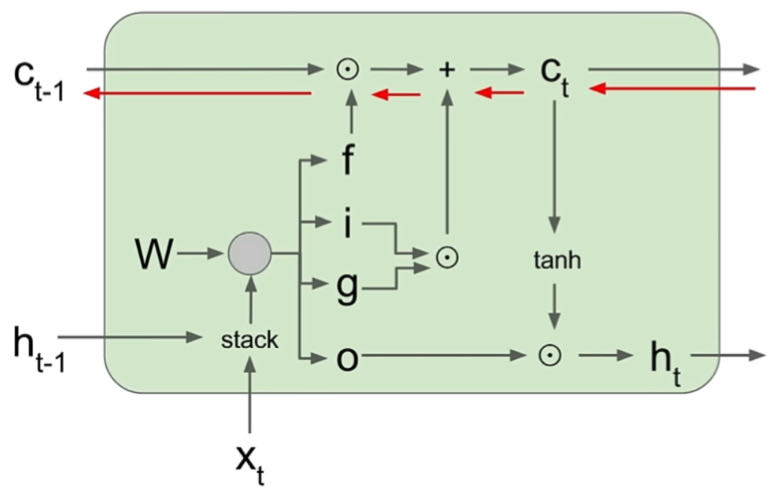
\includegraphics[width=0.4\textheight]{./figures/lstmarchitecture.jpg}
        \caption{LSTM结构}
        \label{fig:lstmarchitecture}
    \end{figure}

    LSTM的训练过程和RNN类似,同样比较有无调度器情况下模型的训练情况,得到的损失曲线如图\ref{fig:lstmlosshistory}所示。
    对应的权重矩阵热力图和文本生成结果参见附录。

    \begin{figure}[H]
        \centering
        \begin{subfigure}{0.45\textwidth}
            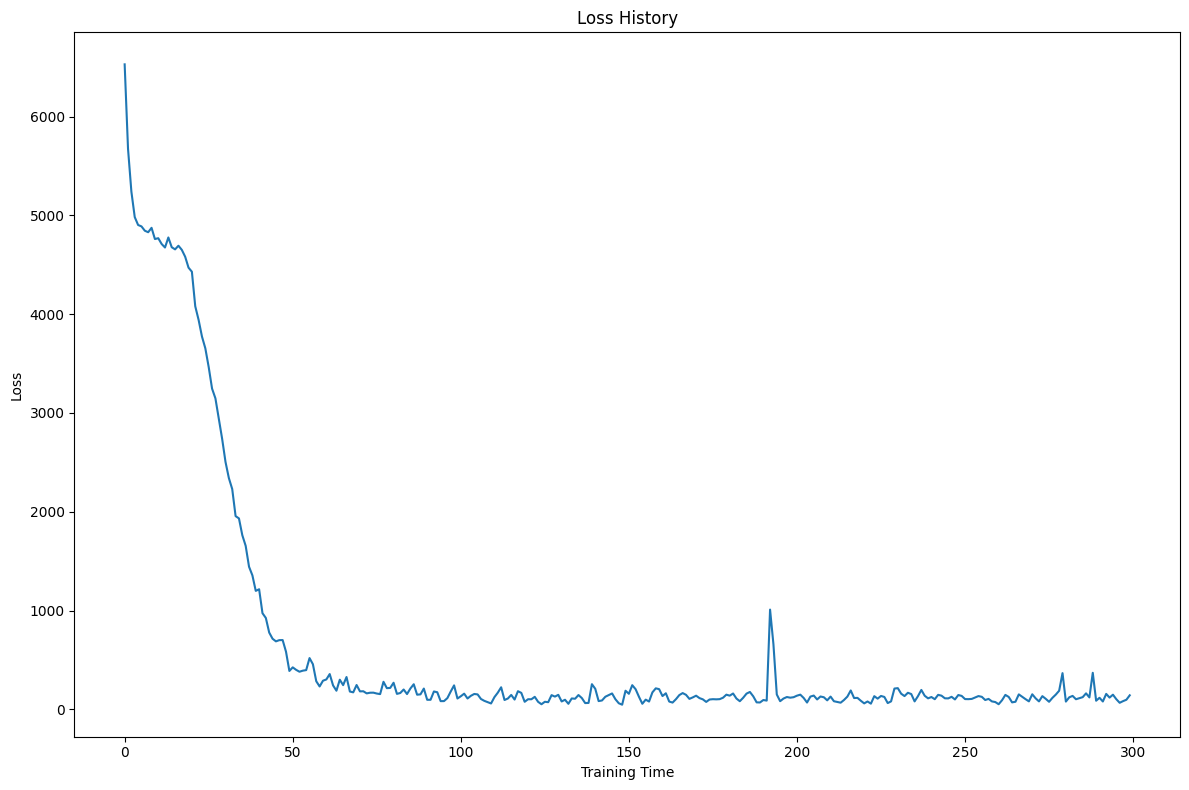
\includegraphics[width=\linewidth]{../output/lstm/no scheduler/lstm_loss.png}
            \caption{不使用调度器}
            \label{fig:LSTMlosshistorynoscheduler}
        \end{subfigure}
        \hfill
        \begin{subfigure}{0.45\textwidth}
            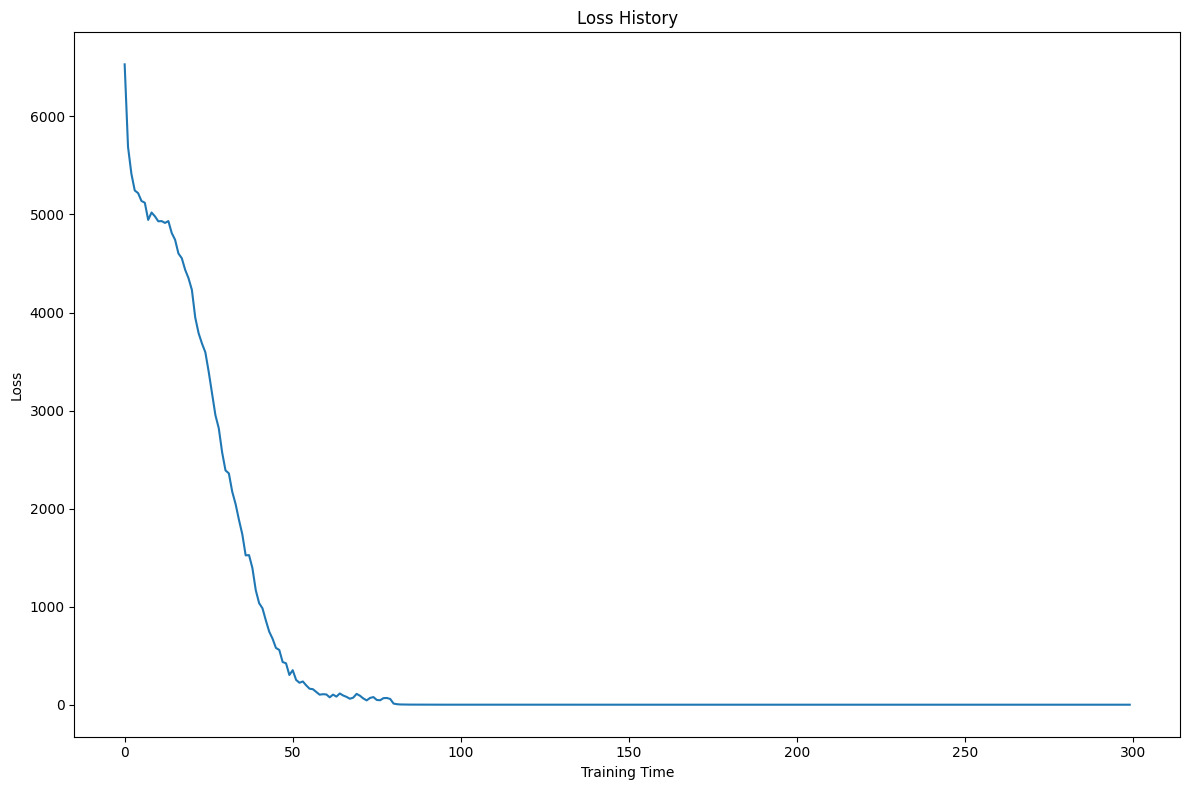
\includegraphics[width=\linewidth]{../output/lstm/with scheduler/lstm_loss.png}
            \caption{使用调度器}
            \label{fig:LSTMlosshistorywithscheduler}
        \end{subfigure}
        \caption{LSTM损失曲线}
        \label{fig:lstmlosshistory}
    \end{figure}

    可以发现,LSTM损失值收敛的速度快于RNN,并且最终收敛的值也远小于RNN的收敛值。
    两者生成的文本中的语法错误数量基本相同。在忽略标点符号以及大小写的情况下,
    不使用调度器时错误数量约为4至6处,使用调度器时错误数量约为2至3处。
	\section{Transformer}

Transformer整体架构如图\ref{fig:TransformerArchitecture}和\ref{fig:transformermechanism}所示,包括编码器和解码器两个部分。
每个部分由多个相同的层堆叠而成,其中最核心的组件是注意力机制和多头注意力机制。
\begin{figure}
    \centering
    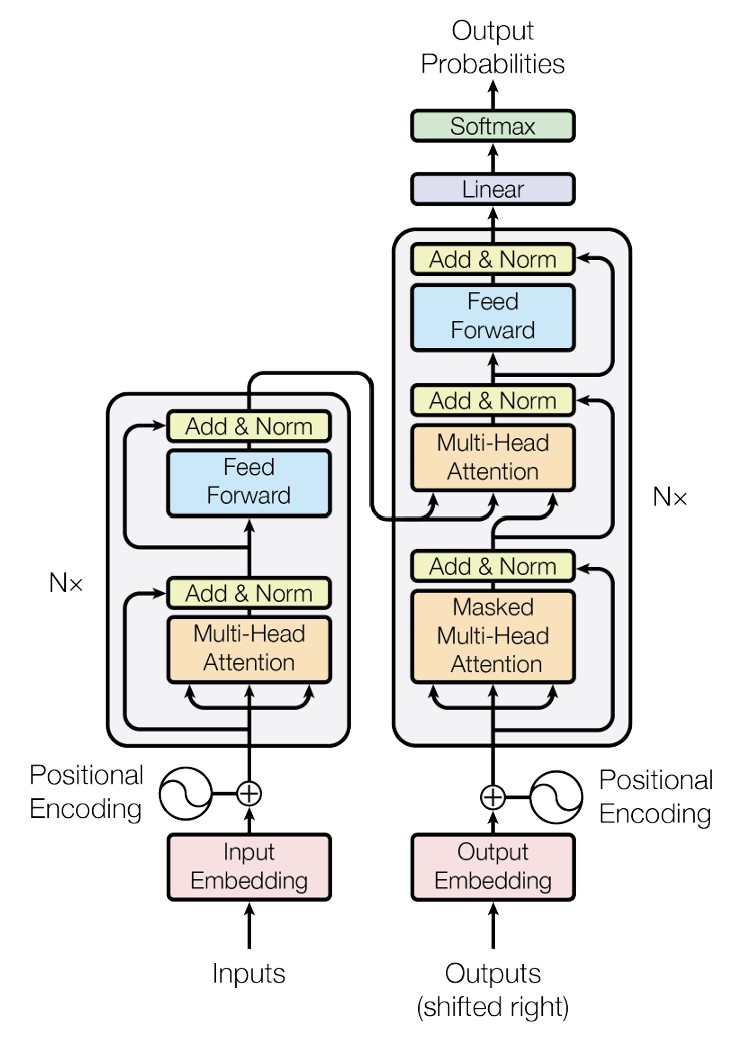
\includegraphics[width=0.3\linewidth]{./figures/TransformerArchitecture.jpg}
    \caption{Transformer整体架构}
    \label{fig:TransformerArchitecture}
\end{figure}

\begin{figure}[H]
    \centering
    \begin{subfigure}[b]{0.45\textwidth}
        \centering
        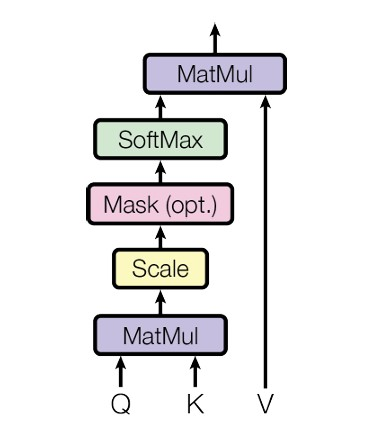
\includegraphics[width=0.5\linewidth]{./figures/ScaledDotProductAttention.jpg}
        \caption{注意力机制}
        \label{fig:ScaledDotProductAttention}
    \end{subfigure}
    \hfill
    \begin{subfigure}[b]{0.45\textwidth}
        \centering
        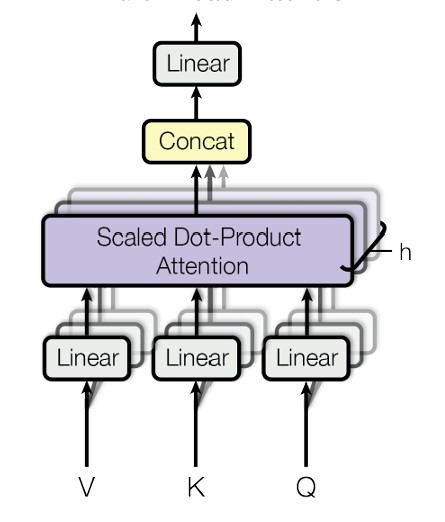
\includegraphics[width=0.5\linewidth]{./figures/MultiHeadAttetion.jpg}
        \caption{多头注意力机制}
        \label{fig:MultiHeadAttetion}
    \end{subfigure}
    \caption{Transformer机制图}
    \label{fig:transformermechanism}
\end{figure}

注意力机制通过计算输入序列中不同元素之间的相关性来为每个元素分配不同的权重。
其核心计算过程是缩放点积注意力(Scaled Dot-Product Attention),
如图\ref{fig:ScaledDotProductAttention}所示。
对于查询向量$\mathbf{Q}$,键向量$\mathbf{K}$,和值向量$\mathbf{V}$,其计算公式为:

\begin{equation}
    \text{Attention}(\mathbf{Q}, \mathbf{K}, \mathbf{V}) = \text{softmax}\left(\frac{\mathbf{QK}^T}{\sqrt{d_k}}\right)\mathbf{V}
\end{equation}
其中,$d_k$是键向量的维度,用于缩放点积以避免数值过大。

多头注意力机制是对注意力机制的扩展,它通过将输入序列映射到多个不同的子空间来捕获更多的特征,如图\ref{fig:MultiHeadAttetion}所示。
具体来说,输入$\mathbf{Q}$, $\mathbf{K}$, $\mathbf{V}$分别经过线性变换生成多个头,
每个头都执行独立的缩放点积注意力,然后将各头的输出拼接并通过线性变换得到最终输出:

\begin{equation}
    \text{MultiHead}(\mathbf{Q}, \mathbf{K}, \mathbf{V}) = \text{Concat}(\text{head}_1, \ldots, \text{head}_h)\mathbf{W}^O
\end{equation}
其中每个头的计算为:

\begin{equation}
    \text{head}_i = \text{Attention}(\mathbf{Q}\mathbf{W}_i^Q, \mathbf{K}\mathbf{W}_i^K, \mathbf{V}\mathbf{W}_i^V)
\end{equation}

由于Transformer不包含循环结构,为了引入序列信息,
位置编码(Positional Encoding)被添加到输入序列中。
位置编码是预先定义的,常用的是正弦和余弦函数生成的编码:

\begin{equation}
    \begin{aligned}
        \text{PE}_{(pos, 2i)} = \sin\left(\frac{pos}{10000^{2i/d_{model}}}\right)\\
        \text{PE}_{(pos, 2i+1)} = \cos\left(\frac{pos}{10000^{2i/d_{model}}}\right)
    \end{aligned}
\end{equation}
其中$pos$是位置,$i$是维度索引,$d_{model}$是模型的维度。

本次实验中的所构建的模型编码器和解码器的层数均为6层,原始输入与RNN相同,
训练过程的损失曲线如图\ref{fig:TransformerLossHistory}所示,
模型各层权重矩阵可视化结果以及文本生成结果见附录。
其中不使用调度器时损失值收敛于0.0049,使用调度器时损失值收敛于0.0091。
\begin{figure}[H]
    \centering
    \begin{subfigure}[b]{0.45\textwidth}
        \centering
        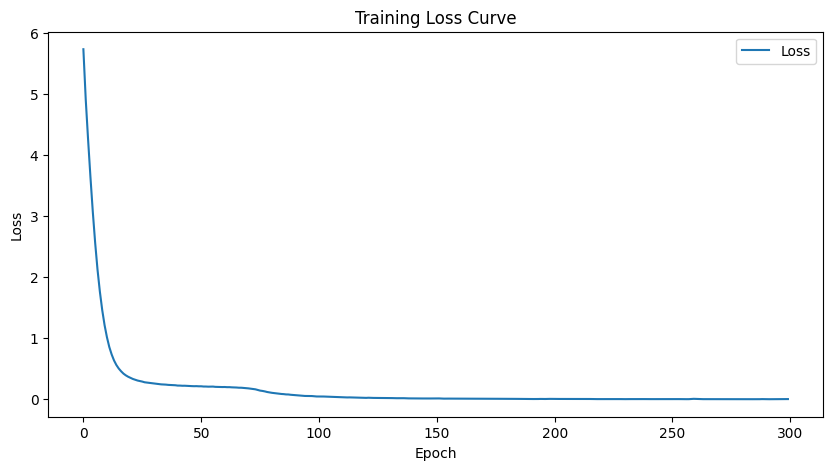
\includegraphics[width=\linewidth]{../output/transformer/no scheduler/loss history.png}
        \caption{不使用调度器}
        \label{fig:TransformerLossHistorynoscheduler}
    \end{subfigure}
    \hfill
    \begin{subfigure}[b]{0.45\textwidth}
        \centering
        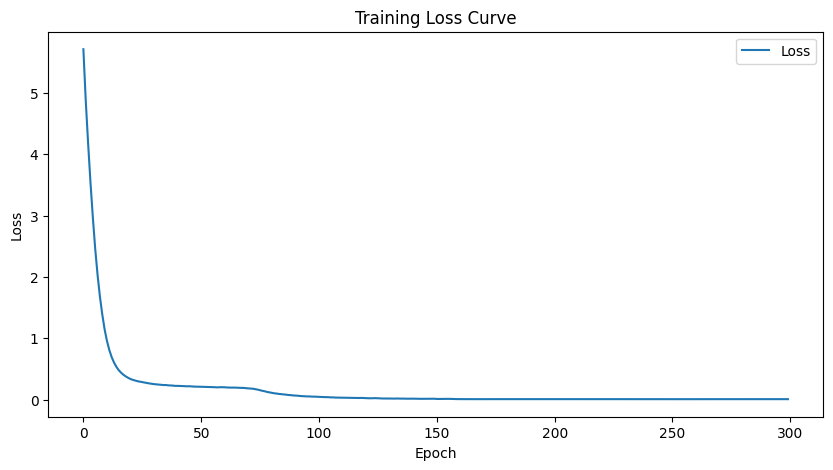
\includegraphics[width=\linewidth]{../output/transformer/with scheduler/loss history.png}
        \caption{使用调度器}
        \label{fig:TransformerLossHistorywithscheduler}
    \end{subfigure}
    \caption{损失曲线}
    \label{fig:TransformerLossHistory}
\end{figure}

  \section{附录}

\subsection{LSTM}

\begin{figure}[H]
    \centering
    \begin{subfigure}{0.3\textwidth}
        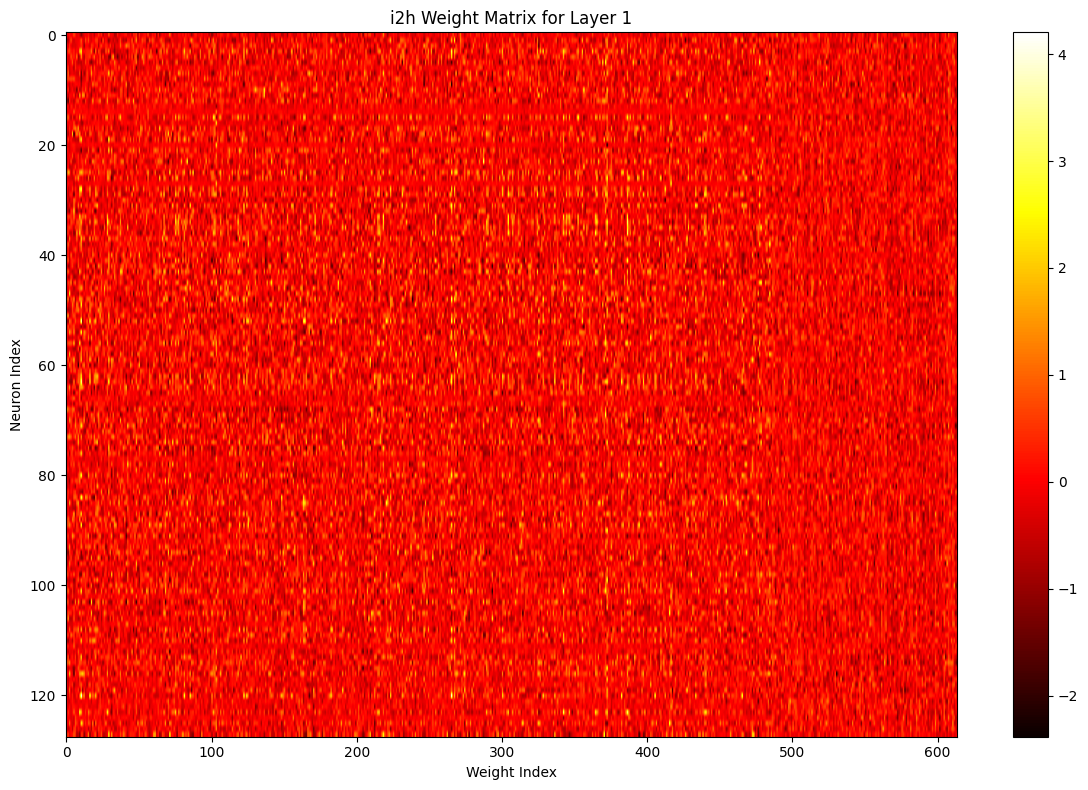
\includegraphics[width=\linewidth]{../output/lstm/no scheduler/i2h Weight Matrix for Layer 1.png}
        \caption{第1层}
        \label{fig:lstmweightmatrixforlayer1noscheduler}
    \end{subfigure}
    \hfill
    \begin{subfigure}{0.3\textwidth}
        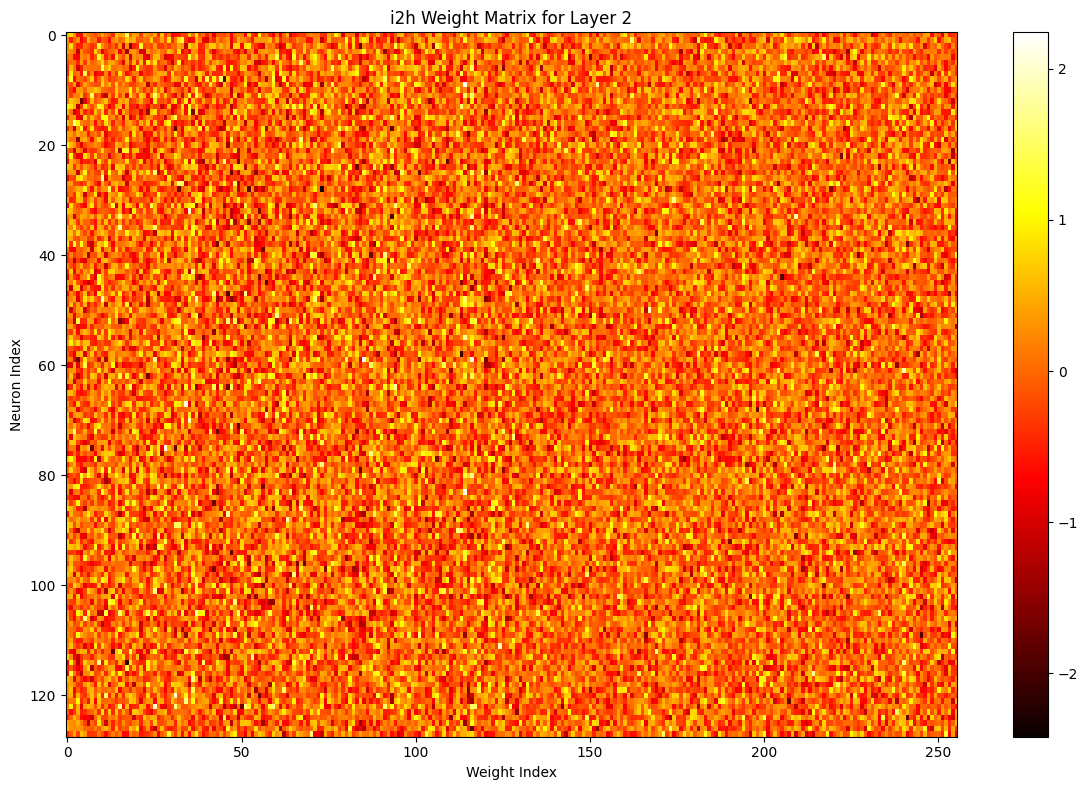
\includegraphics[width=\linewidth]{../output/lstm/no scheduler/i2h Weight Matrix for Layer 2.png}
        \caption{第2层}
        \label{fig:lstmweightmatrixforlayer2noscheduler}
    \end{subfigure}
    \hfill
    \begin{subfigure}{0.3\textwidth}
        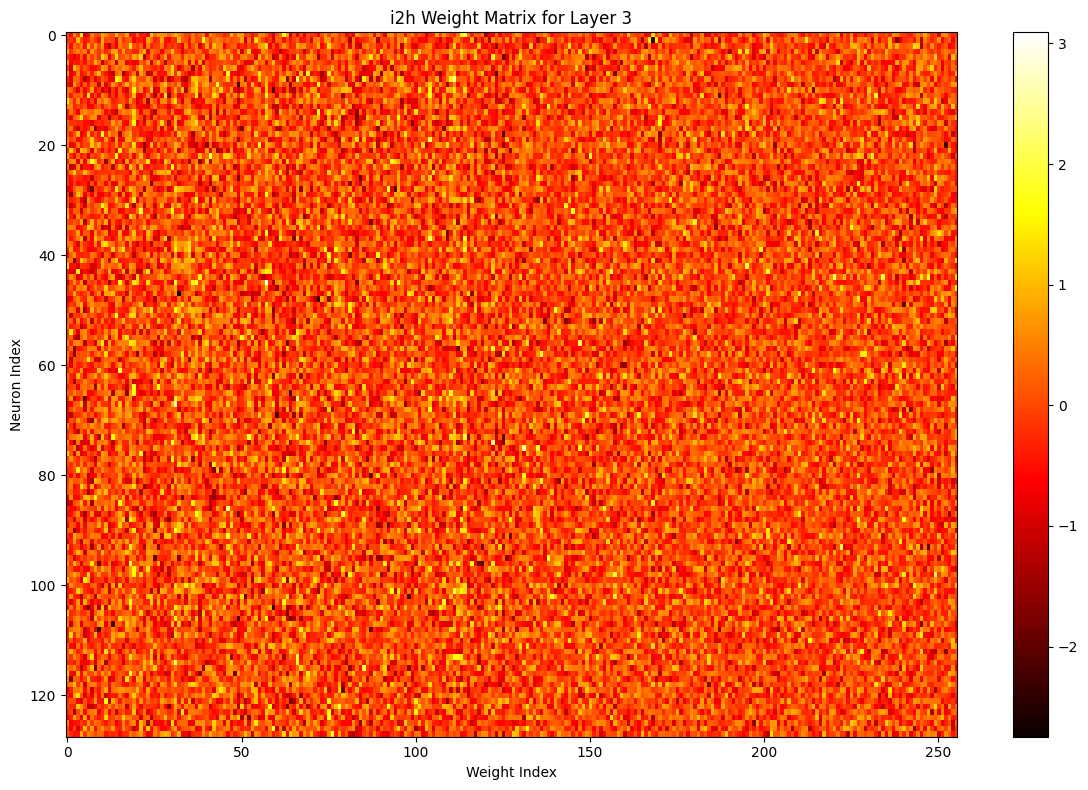
\includegraphics[width=\linewidth]{../output/lstm/no scheduler/i2h Weight Matrix for Layer 3.png}
        \caption{第3层}
        \label{fig:lstmweightmatrixforlayer3noscheduler}
    \end{subfigure}
    \caption{LSTM隐藏层权重矩阵(不使用调度器)}
    \label{fig:lstmweightmatrixnoscheduler}
\end{figure}

\begin{figure}[H]
    \centering
    \begin{subfigure}{0.3\textwidth}
        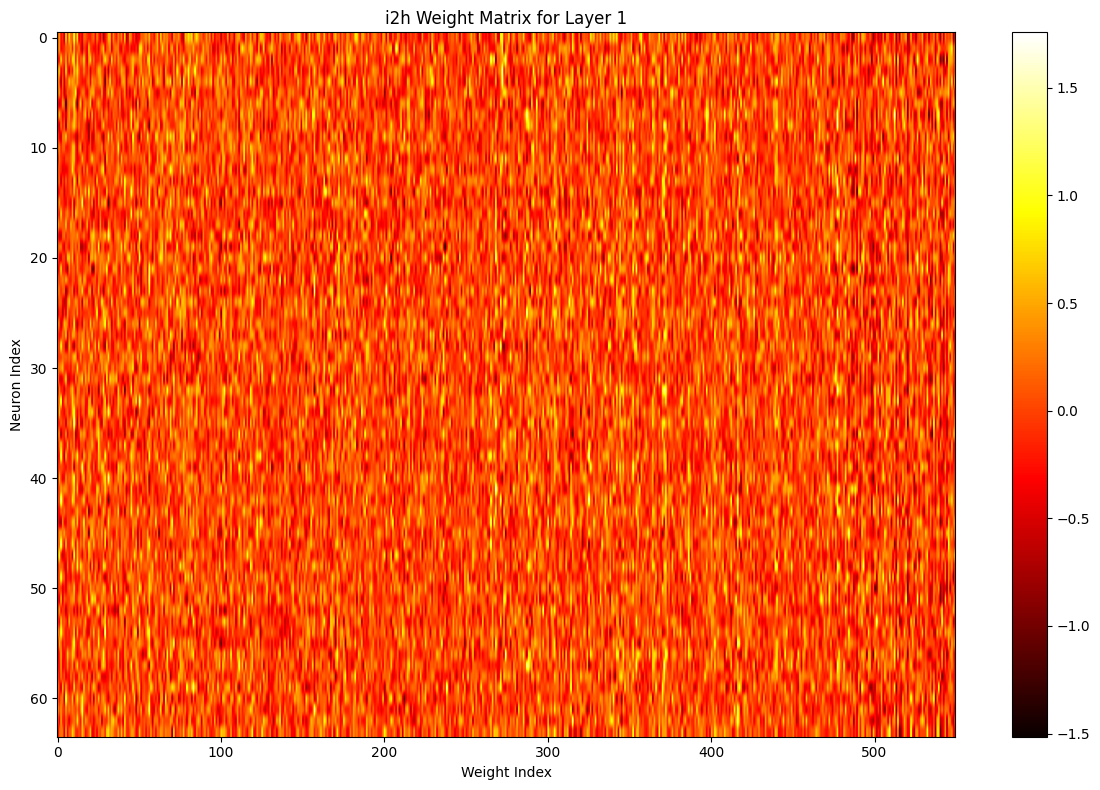
\includegraphics[width=\linewidth]{../output/lstm/with scheduler/i2h Weight Matrix for Layer 1.png}
        \caption{第1层}
        \label{fig:lstmweightmatrixforlayer1withscheduler}
    \end{subfigure}
    \hfill
    \begin{subfigure}{0.3\textwidth}
        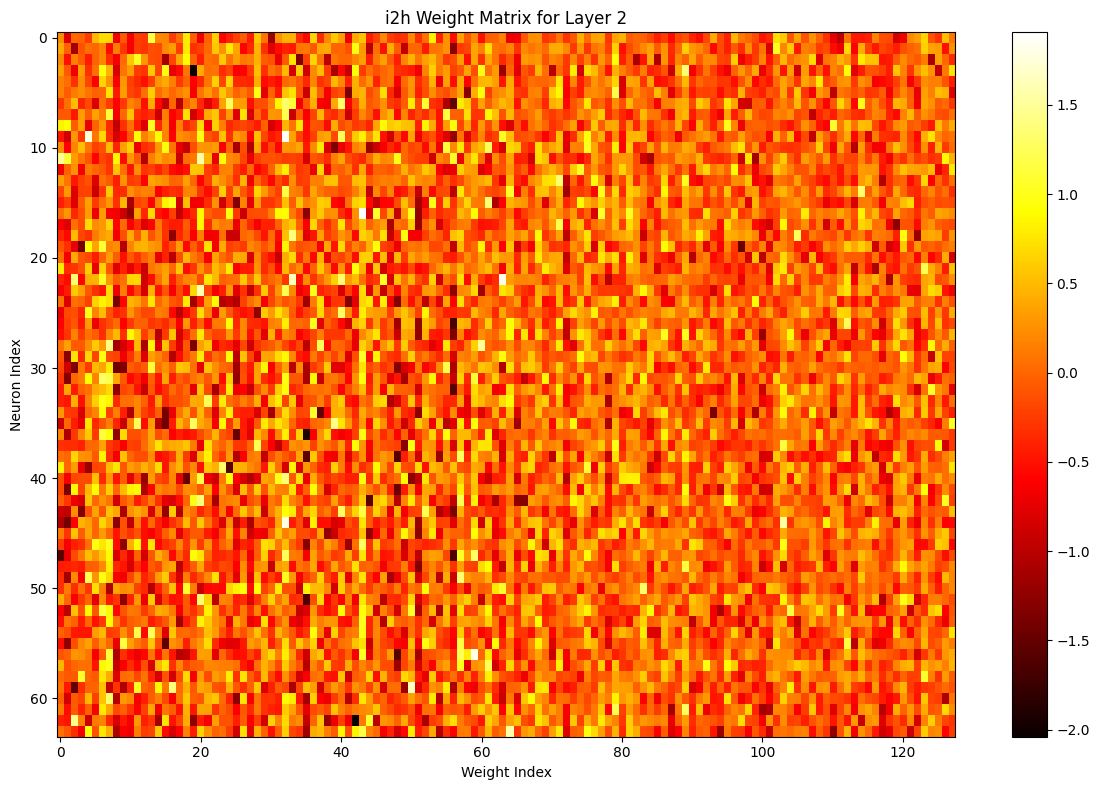
\includegraphics[width=\linewidth]{../output/lstm/with scheduler/i2h Weight Matrix for Layer 2.png}
        \caption{第2层}
        \label{fig:lstmweightmatrixforlayer2withscheduler}
    \end{subfigure}
    \hfill
    \begin{subfigure}{0.3\textwidth}
        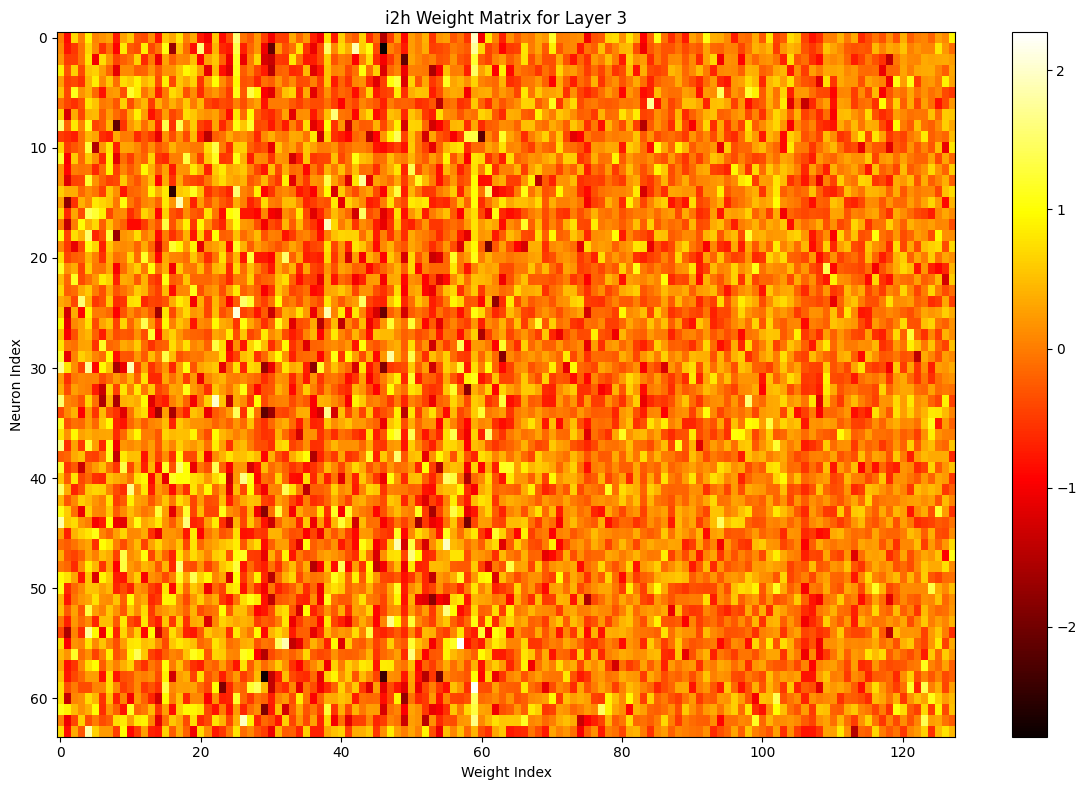
\includegraphics[width=\linewidth]{../output/lstm/with scheduler/i2h Weight Matrix for Layer 3.png}
        \caption{第3层}
        \label{fig:lstmweightmatrixforlayer3withscheduler}
    \end{subfigure}
    \caption{LSTM隐藏层权重矩阵(使用调度器)}
    \label{fig:lstmweightmatrixwithscheduler}
\end{figure}

\begin{figure}[H]
    \centering
    \begin{subfigure}[b]{0.45\textwidth}
        \textit{"china has an important pool of the indonesia center for middle east studies told china daily that the success of 14 palestinian factions including hamas and fatah in reaching an agreement is due to chinas impartial efforts which provide space for the palestinian people to formulate what is best for them while fostering new quality productive forces by giving play to the leading role of enterprises in scitech innovation and stimulating their innovation vitality he said this highly innovation the country can accelerate the development of the declaration by palestinian factions un spokesman stephane dujarric said in new york on tuesday"}
        \caption{不使用调度器}
        \label{fig:lstmtextnoscheduler}
    \end{subfigure}
    \hfill
    \begin{subfigure}[b]{0.45\textwidth}
        \textit{"china signing of the declaration aimed at achieving national unity according to turkiyes anadolu agency while welcoming the declaration the sultanate of oman said this highly needed goal should be achieved by adhering to relevant resolutions of international legitimacy according to the oman news agency dina yulianti sulaeman director of the indonesia center for middle east studies told china daily that the success of 14 palestinian factions including hamas and fatah in reaching an agreement is due to chinas impartial efforts which provide space for the palestinian people to formulate what is best for them while fostering new quality productive forces"}
        \caption{使用调度器}
        \label{fig:lstmtextwithscheduler}
    \end{subfigure}
    \caption{LSTM生成文本比较}
    \label{fig:lstmtext-comparison}
\end{figure}

\subsection{Transformer}

\begin{figure}[H]
    \centering
    \begin{subfigure}[c]{0.45\textwidth}
        \centering
        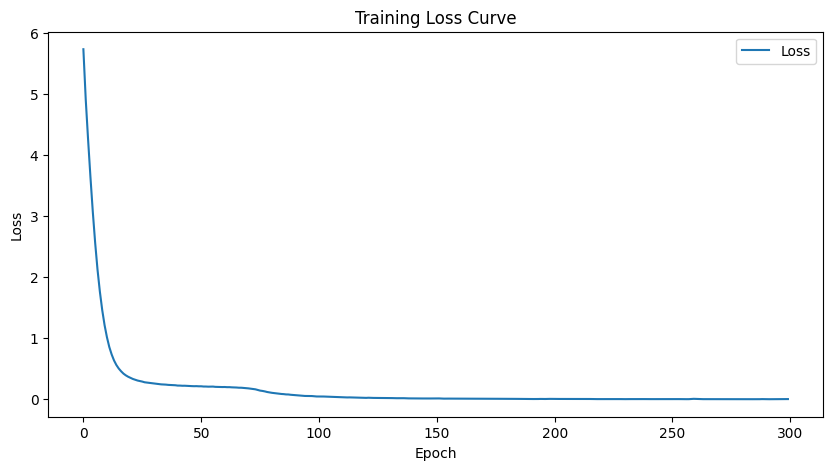
\includegraphics[width=\textwidth]{../output/transformer/no scheduler/loss history.png}
        \caption{不使用调度器}
    \end{subfigure}
    \hfill
    \begin{subfigure}[c]{0.45\textwidth}
        \centering
        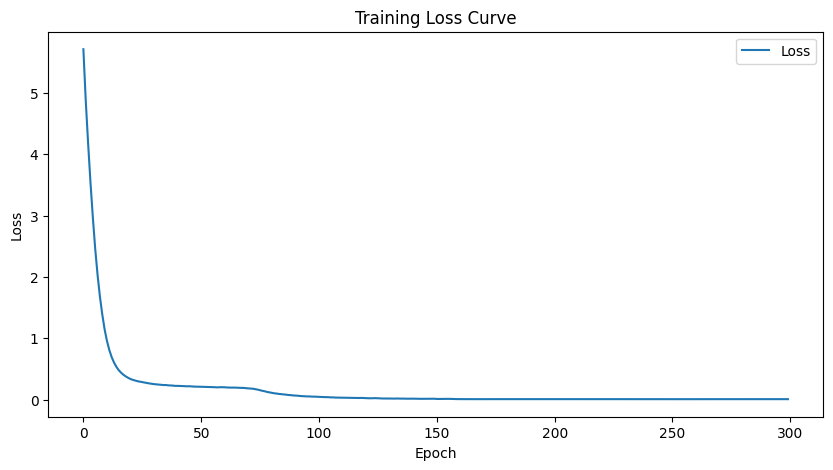
\includegraphics[width=\textwidth]{../output/transformer/with scheduler/loss history.png}
        \caption{使用调度器}
    \end{subfigure}
    \caption{损失曲线}
\end{figure}

\begin{figure}[H]
    \centering
    \begin{subfigure}{0.3\textwidth}
        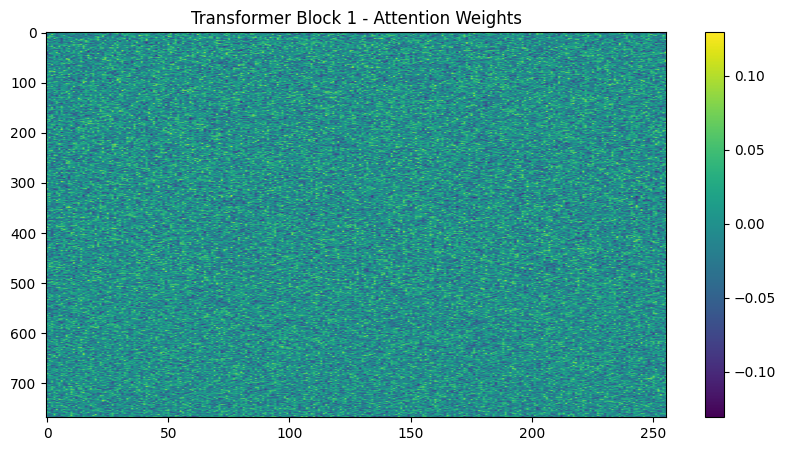
\includegraphics[width=\linewidth]{../output/transformer/no scheduler/Transformer Block 1 Attention Weights.png}
        \caption{第1层}
        \label{fig:transformerblock1attentionweightsnoscheduler}
    \end{subfigure}
    \hfill
    \begin{subfigure}{0.3\textwidth}
        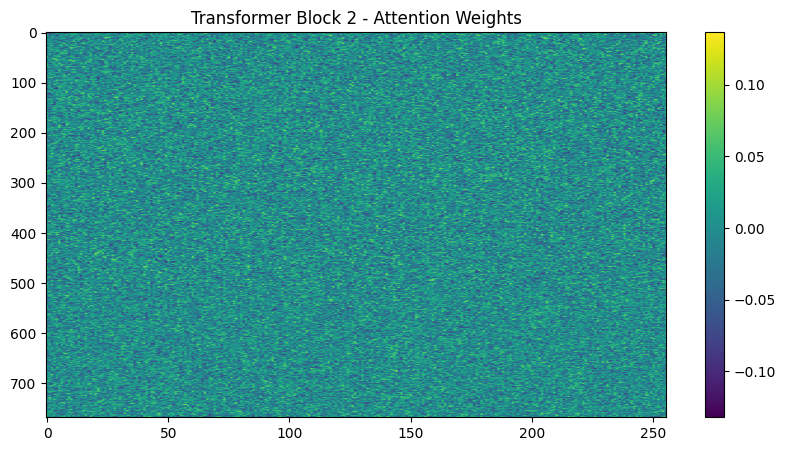
\includegraphics[width=\linewidth]{../output/transformer/no scheduler/Transformer Block 2 Attention Weights.png}
        \caption{第2层}
        \label{fig:transformerblock2attentionweightsnoscheduler}
    \end{subfigure}
    \hfill
    \begin{subfigure}{0.3\textwidth}
        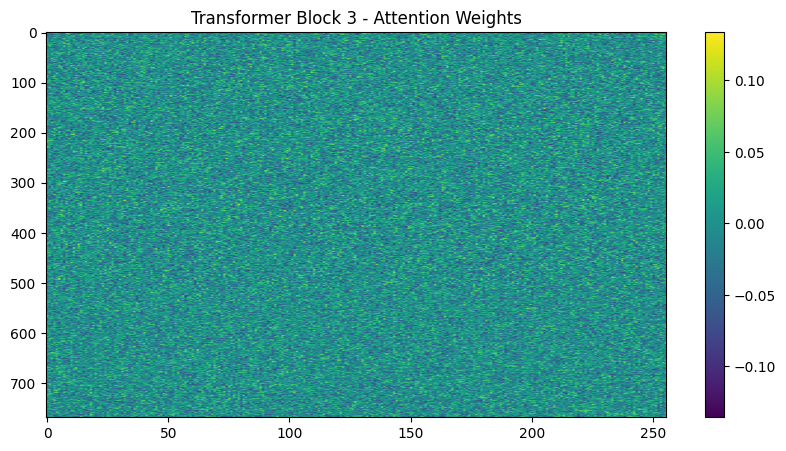
\includegraphics[width=\linewidth]{../output/transformer/no scheduler/Transformer Block 3 Attention Weights.png}
        \caption{第3层}
        \label{fig:transformerblock3attentionweightsnoscheduler}
    \end{subfigure}

    \vfill

    \begin{subfigure}{0.3\textwidth}
        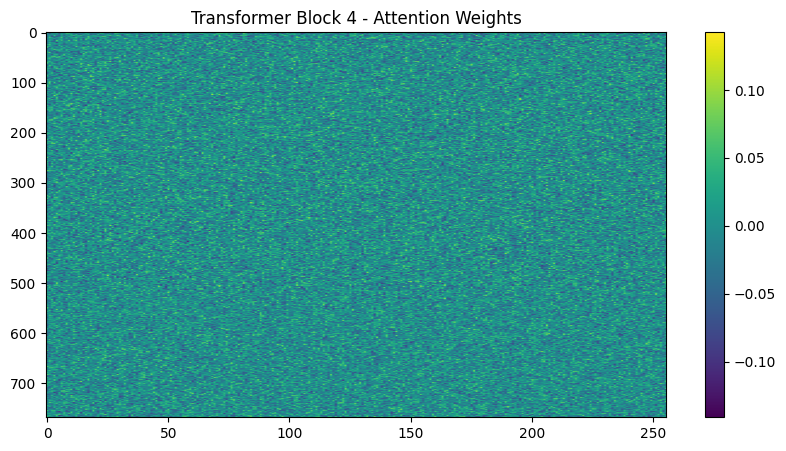
\includegraphics[width=\linewidth]{../output/transformer/no scheduler/Transformer Block 4 Attention Weights.png}
        \caption{第4层}
        \label{fig:transformerblock4attentionweightsnoscheduler}
    \end{subfigure}
    \hfill
    \begin{subfigure}{0.3\textwidth}
        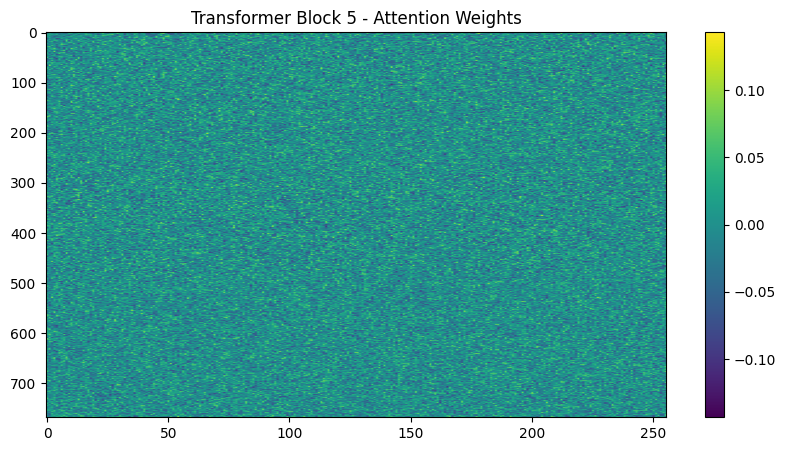
\includegraphics[width=\linewidth]{../output/transformer/no scheduler/Transformer Block 5 Attention Weights.png}
        \caption{第5层}
        \label{fig:transformerblock5attentionweightsnoscheduler}
    \end{subfigure}
    \hfill
    \begin{subfigure}{0.3\textwidth}
        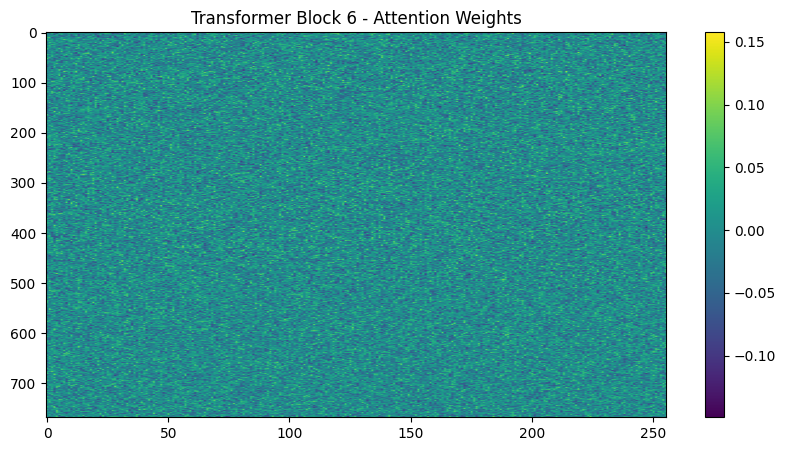
\includegraphics[width=\linewidth]{../output/transformer/no scheduler/Transformer Block 6 Attention Weights.png}
        \caption{第6层}
        \label{fig:transformerblock6attentionweightsnoscheduler}
    \end{subfigure}

    \caption{Transformer注意力权重矩阵热力图(不使用调度器)}
    \label{fig:transformerattentionweightsnoscheduler}
\end{figure}

\begin{figure}[H]
    \centering
    \begin{subfigure}{0.3\textwidth}
        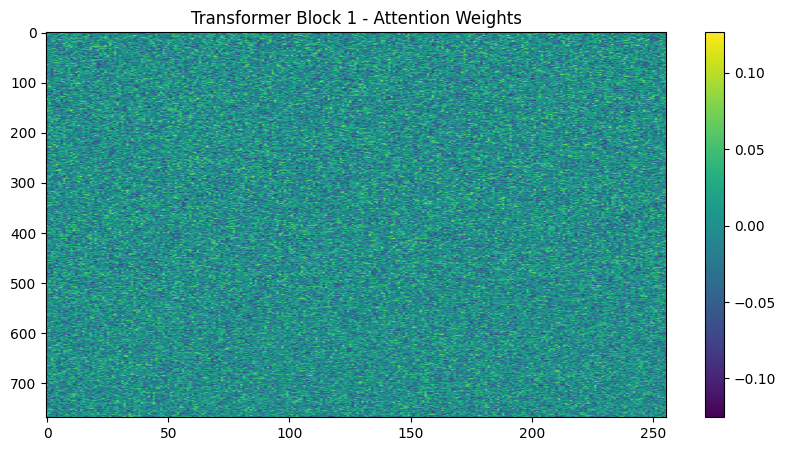
\includegraphics[width=\linewidth]{../output/transformer/with scheduler/Transformer Block 1 Attention Weights.png}
        \caption{第1层}
        \label{fig:transformerblock1attentionweightswithscheduler}
    \end{subfigure}
    \hfill
    \begin{subfigure}{0.3\textwidth}
        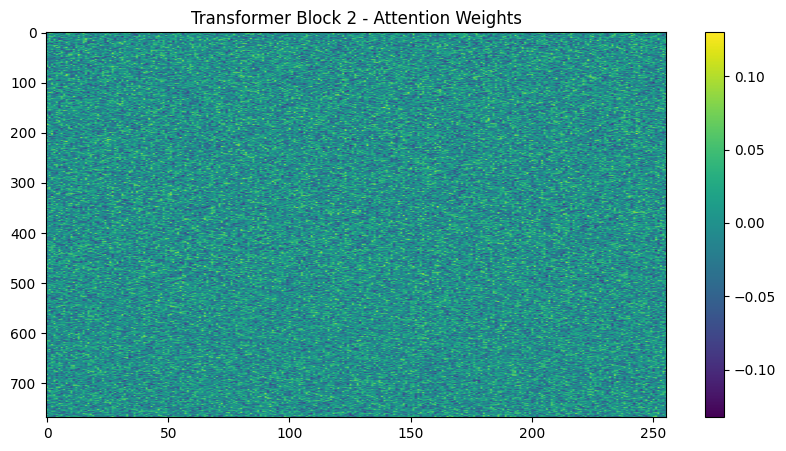
\includegraphics[width=\linewidth]{../output/transformer/with scheduler/Transformer Block 2 Attention Weights.png}
        \caption{第2层}
        \label{fig:transformerblock2attentionweightswithscheduler}
    \end{subfigure}
    \hfill
    \begin{subfigure}{0.3\textwidth}
        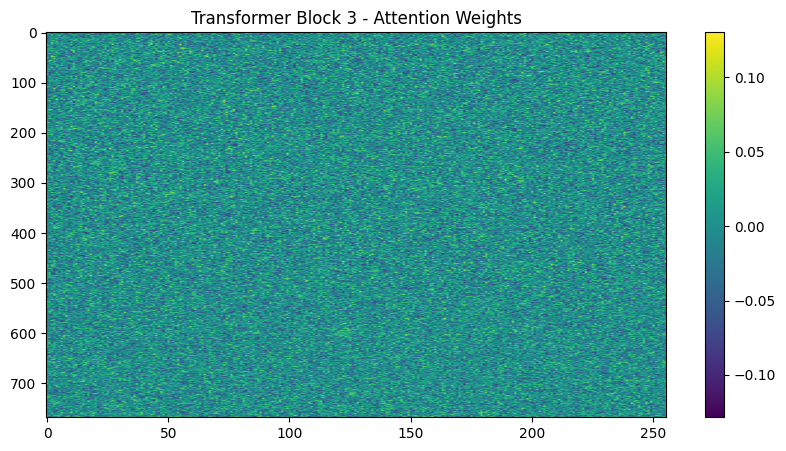
\includegraphics[width=\linewidth]{../output/transformer/with scheduler/Transformer Block 3 Attention Weights.png}
        \caption{第3层}
        \label{fig:transformerblock3attentionweightswithscheduler}
    \end{subfigure}

    \vfill

    \begin{subfigure}{0.3\textwidth}
        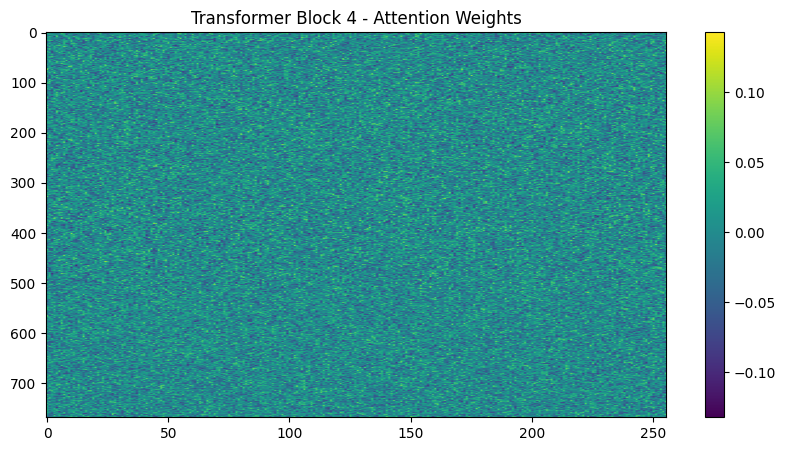
\includegraphics[width=\linewidth]{../output/transformer/with scheduler/Transformer Block 4 Attention Weights.png}
        \caption{第4层}
        \label{fig:transformerblock4attentionweightswithscheduler}
    \end{subfigure}
    \hfill
    \begin{subfigure}{0.3\textwidth}
        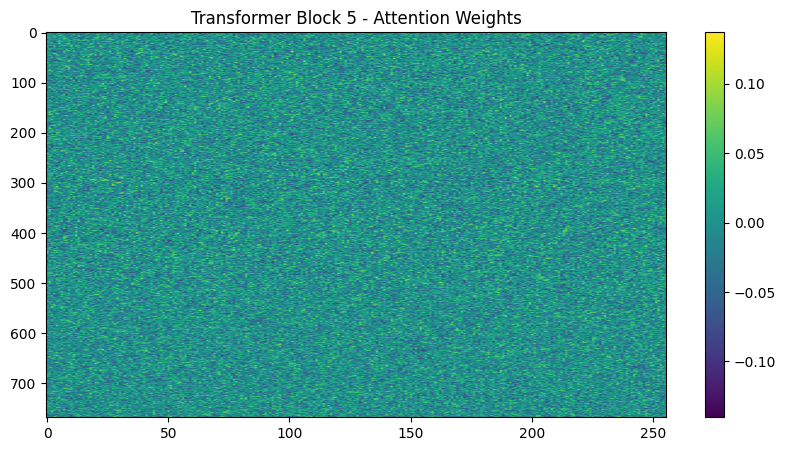
\includegraphics[width=\linewidth]{../output/transformer/with scheduler/Transformer Block 5 Attention Weights.png}
        \caption{第5层}
        \label{fig:transformerblock5attentionweightswithscheduler}
    \end{subfigure}
    \hfill
    \begin{subfigure}{0.3\textwidth}
        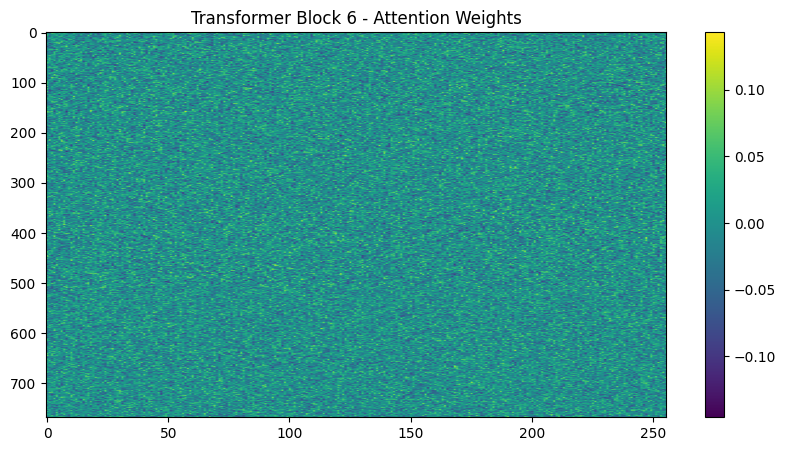
\includegraphics[width=\linewidth]{../output/transformer/with scheduler/Transformer Block 6 Attention Weights.png}
        \caption{第6层}
        \label{fig:transformerblock6attentionweightswithscheduler}
    \end{subfigure}

    \caption{Transformer注意力权重矩阵热力图(使用调度器)}
    \label{fig:transformerattentionweightswithscheduler}
\end{figure}

\begin{figure}[H]
    \centering
    \begin{subfigure}[b]{0.45\textwidth}
        \textit{"china china china china china china challenges china china china china china china china china china china china china china to better leverage to better leverage be realistic to better leverage their financial resources for supporting innovations while fostering to better balance spending responsibilities between local and central governments encouraging the development of venture capital and patient capital will be important improvements he said li dongsheng founder and chairman of chinese consumer electronics maker tcl technology group corp said chinas new growth drivers come from industrial transformation and technological innovation the country can accelerate the formation of sound systems and mechanisms"}
        \caption{不使用调度器}
        \label{fig:transformertextnoscheduler}
    \end{subfigure}
    \hfill
    \begin{subfigure}[b]{0.45\textwidth}
        \textit{"china china china china china china china china china china china china china china china china china china china china china china china daily that china daily that china daily that china daily that china is an important role in an opportunity china daily that china daily that china daily that china daily that china daily that china daily that china daily that china daily that central committee that china daily that china daily that china daily that china daily that china daily that china daily that china daily that china daily that china china daily that china an china daily"}
        \caption{使用调度器}
        \label{fig:transformertextwithscheduler}
    \end{subfigure}
    \caption{Transformer生成文本比较}
    \label{fig:transformer-comparison}
\end{figure}
	
\end{document}
